% paper/sections/scaling_laws.tex -- Pillar 1 (GRPO saturation / scaling law analysis)
% Canonical saturation fit R(t) = R_max * (1 - exp(-lambda * t)) across the
% five frontier-scale anchors (Qwen3.5-4B, Qwen3-8B, Llama-3.1-8B-Instruct,
% DeepSeek-V3.1, Nemotron-120B), plus an OLS-based cross-scale law over
% log_10(N).  Elevation diagnostics (iter 9):
%   scripts/scaling_law_elevated.py produces
%     experiments/results/scaling_law_bootstrap_ci.tsv
%     experiments/results/scaling_law_holdout.tsv
%     experiments/results/scaling_law_compute.tsv
%     experiments/results/scaling_law_nemotron_rootcause.tsv
%     figures/scaling_law_elevated.{pdf,png}
% Original canonical analysis: scripts/scaling_law_fit.py -> scaling_law_fits.tsv,
% scaling_law_three_phase.tsv, scaling_law_cross_scale.tsv.

\paragraph{Saturation model across the 4B--671B range.}
\label{par:saturation}
We fit the canonical saturation model
\begin{equation}
  \label{eq:sat}
  R(t) = R_{\max}\bigl(1 - e^{-\lambda t}\bigr),
  \qquad t = 1, \dots, T,
\end{equation}
to per-step reward traces from each frontier-scale
\textsc{tinker} run and report the ceiling $R_{\max}$, the
learning rate $\lambda$, and the saturation time
$t_{80} = -\ln(0.2)/\lambda$ at which the trace first crosses
$0.8\,R_{\max}$.  The model follows
\textsc{nimmaturi}-style notation~\citep{nimmaturi2025predictive},
which postulates a slow-start $\to$ rapid-improvement $\to$
plateau template for GRPO learning curves.

\begin{table}[t]
  \centering
  \small
  \begin{tabular}{lrrrrrrrrl}
    \toprule
    Model & $N$ (B) & $n$ & mean $R$ & peak $R$ &
           $\bar R_{\text{early}} \!\to\! \bar R_{\text{late}}$ &
           $\hat \beta_{\text{OLS}}$ &
           $R_{\max}$ & $\lambda$ & Phase \\
    \midrule
    Qwen3.5-4B             &   4.0 & 30 & 0.817 & 1.000 & 0.813 $\to$ 0.850 & $+0.0001$ & 0.817 & $10.0^{\dagger}$ & plateau \\
    Qwen3-8B               &   8.0 & 30 & 0.285 & 0.625 & 0.244 $\to$ 0.344 & $+0.0032$ & 0.285 & $10.0^{\dagger}$ & saturation \\
    Llama-3.1-8B-Instruct  &   8.0 & 30 & 0.869 & 1.000 & 0.925 $\to$ 0.844 & $-0.0037$ & 0.869 & $10.0^{\dagger}$ & drift \\
    DeepSeek-V3.1          & 671.0 & 20 & 0.844 & 1.000 & 0.833 $\to$ 0.813 & $+0.0001$ & 0.844 & $10.0^{\dagger}$ & plateau \\
    Nemotron-120B          & 120.0 & 20 & 0.175 & 0.875 & 0.146 $\to$ 0.208 & $+0.0026$ & 0.182 & \textbf{0.99} & \textbf{collapse} \\
    \bottomrule
  \end{tabular}
  \caption{\textbf{Saturation-model fits across 4B--671B.}
    $\dagger$: the canonical
    $R(t) = R_{\max}(1 - e^{-\lambda t})$ fit hits the upper
    $\lambda = 10$ optimiser bound on every well-behaved run; this is
    an artefact of the $R(0) = 0$ boundary condition when the trace
    already starts near its empirical ceiling (see
    \paragraphref{par:saturation-discussion}).
    $\hat \beta_{\text{OLS}}$ is the per-step OLS slope of $R(t)$ vs.~$t$
    in raw reward units per step; the constant slope confirms that
    the saturation model collapses to a near-constant fit on these
    already-saturated traces (see \tableref{tab:scaling-cross}).
    Bold $\lambda$ and Phase identify the only run whose $\lambda$
    leaves the bound and where the late-window mean falls below
    $0.4\times$ peak -- the three-phase ``collapse'' criterion.}
  \label{tab:scaling-fits}
\end{table}

\paragraph{Where the model fits and where it does not.}
\label{par:saturation-discussion}
The raw saturation model collapses to the $\lambda = 10$ upper bound
on four of five runs (Table~\ref{tab:scaling-fits}).  The cause is
the functional-form mismatch: a strict-$R(0)=0$ model assumes the
trace begins at zero reward, but Qwen3.5-4B starts at $R(1)=1.0$,
Llama-3.1-8B-Instruct at $R(1)=1.0$, and DeepSeek-V3.1 at
$R(1)=0.875$.  When the trace is already at or above its eventual
ceiling, the optimiser makes $\lambda$ as large as allowed so that
$R_{\max}(1 - e^{-10 t}) \approx R_{\max}$ for $t \ge 1$, which
yields $t_{80} \approx -\ln(0.2)/10 \approx 0.16$ step -- a
meaningless artefact, not evidence of instant learning.

The right resolution is two separate diagnostics, both reported
here:

\begin{enumerate}
  \item \emph{Per-step OLS slope} $\hat\beta_{\text{OLS}}$ of
    $R(t)$ vs.~$t$ (Table~\ref{tab:scaling-fits}, column~7).
    Across the four well-behaved runs
    $|\hat\beta_{\text{OLS}}| \le 0.0037$ reward/step (i.e.\ the
    traces are statistically flat within their per-step noise),
    while the collapse run Nemotron-120B still shows $\hat\beta
    = +0.0026$ -- not because it is improving, but because its
    sparse spikes pull the OLS slope upward.
  \item \emph{Cross-scale OLS} of $\bar R$ on $\log_{10} N$
    across the five anchor models.  The result is the headline
    scaling-law coefficient in
    Table~\ref{tab:scaling-cross}.
\end{enumerate}

\paragraph{Cross-scale law.}
\label{par:cross-scale}
We regress each per-trace statistic on $\log_{10} N$
(\(N\) = parameter count in billions) by ordinary least squares and
quote block-bootstrap 95\% confidence intervals
($n_{\text{boot}} \approx 1000$ effective row resamples) on
the slopes.  The fitted coefficients are

\begin{table}[t]
  \centering
  \small
  \begin{tabular}{lrrrrr}
    \toprule
    Metric $y$ & Intercept & Slope / decade &
                  Boot slope mean & Boot 95\% CI &
                  $\rho(\log_{10} N, y)$ \\
    \midrule
    mean reward $\bar R$  & 0.633 & $-0.024$ & $-0.117$ & $[-0.796,\ +0.313]$ & $-0.07$ \\
    peak reward $\hat R$  & 0.846 & $\mathbf{+0.037}$ & $-0.010$ & $[-0.623,\ +0.197]$ & $+0.22$ \\
    var reward $\widehat{\text{Var}}[R]$ & 0.040 & $-0.002$ & $-0.004$ & $[-0.063,\ +0.027]$ & $-0.14$ \\
    \bottomrule
  \end{tabular}
  \caption{\textbf{Cross-scale law: per-trace metric vs.~$\log_{10} N$
    across the five frontier anchors.}
    Ordinary least squares with bootstrap 95\% confidence intervals.
    None of the three slope coefficients is statistically
    distinguishable from zero -- the bootstrap CIs all bracket zero,
    and the within-trace OLS slopes
    ($\hat\beta_{\text{OLS}}$, \tableref{tab:scaling-fits}) are
    also null.  Reading: at this benchmark size ($4\,\text{B}
    \le N \le 671\,\text{B}$, $T\!\le\!30$ steps), the saturation
    model is not detectably scale-dependent, because every
    well-behaved run is already saturated within measurement noise.}
  \label{tab:scaling-cross}
\end{table}

\paragraph{Three-phase learning dynamics.}
\label{par:three-phase}
We apply the \citet{nimmaturi2025predictive} slow start
$\to$ rapid improvement $\to$ plateau template to each trace, with
an additional ``collapse'' class for runs whose peak is not
retained.  Of the five anchors, two fall in \emph{plateau}
(Qwen3.5-4B, DeepSeek-V3.1), one in \emph{saturation} (Qwen3-8B),
one in \emph{drift} (Llama-3.1-8B-Instruct, monotone decline), and
one in \emph{collapse} (Nemotron-120B).  No run satisfies the
textbook three-phase criterion, because none of the five anchors
has a slow-start phase: they all start at or above the eventual
late-window mean.  This is consistent with our earlier
observation that GRPO step-1 rewards are already within
$\pm 0.10$ of the per-trace mean for all but Qwen3-8B and
Nemotron-120B.

\paragraph{Nemotron-120B violates the three-phase hypothesis.}
\label{par:nemotron-collapse}
Following \citet{nimmaturi2025predictive}, the three-phase
template predicts slow start $\to$ rapid improvement $\to$
\emph{plateau}, with collapse as a degenerate tail.  Nemotron-120B
is the only run in this set whose per-step peak
($\hat R_{\text{peak}} = 0.875$, step 3) is followed by a
sustained decay: only $5$ of $20$ steps reach reward $> 0.25$, and
$55\%$ of steps report \emph{zero reward}.  The fitted $\lambda
= 0.99$ and $t_{80} = 1.63$ step are the only identifiable
parameters in Table~\ref{tab:scaling-fits} precisely because the
curve does not asymptote -- a robust monotone saturation model is
the wrong functional form.  We therefore report the late-window
collapse magnitude
$\hat R_{\text{peak}} - \bar R_{\text{late}} = 0.667$ reward units
as the empirical effect size of the violation, and treat this run
as the Pillar-1 counterexample to the three-phase prediction.

Operationally, the Nemotron collapse is exactly the failure mode
that pure-reward saturation fits are silent on: the curve does
\emph{not} settle, it diverges downward, and a benchmark that
relies on a saturation-only diagnostic will miss it.  This
motivates the variance-based \textsc{zvf} gate
(companion paper on ZVF) as a complementary diagnostic: the
zero-reward-fraction for Nemotron-120B is $0.55$, well above any
well-behaved run in this set, and the cross-experiment
\textsc{zvf}-vs-failure map
(companion paper on cross-experiment ZVF) would catch the divergence on
reward \emph{variance} rather than reward \emph{mean}.

\paragraph{Falsifiable prediction.}
\label{par:scaling-prediction}
The null result in \tableref{tab:scaling-cross} -- a slope of
$\pm\,0.04$ per decade on $\bar R$, with CI brackets zero across
roughly $2.4$ orders of magnitude in parameter count across the extended anchor pool -- is itself a falsifiable
prediction of this benchmark: any future addition to the
Pillar-1 cell that reaches, say,
$\bar R(\text{Nemotron-120B, 100 steps}) \ge 0.5$ would refute
the saturation-template behaviour we report here.  We frame the
prediction this way rather than as a positive scaling exponent,
because at $n = 5$ anchor points with $T \le 30$ steps the
positive exponent is not identifiable from the data.

\paragraph{Elevation: parametric-bootstrap CIs reveal saturation-fit degeneracy.}
\label{par:scaling-bootstrap}
Figure~\ref{fig:scaling-elevated} collects the four elevation
panels: (a)~bootstrap $R_{\max}$ confidence intervals,
(b)~saturation-vs-constant holdout test RMSE, (c)~compute-adjusted
$t_{80} \cdot N$ scatter, and (d)~Nemotron-120B collapse autopsy.

\begin{figure}[t]
  \centering
  \IfFileExists{figures/scaling_law_elevated.png}{%
  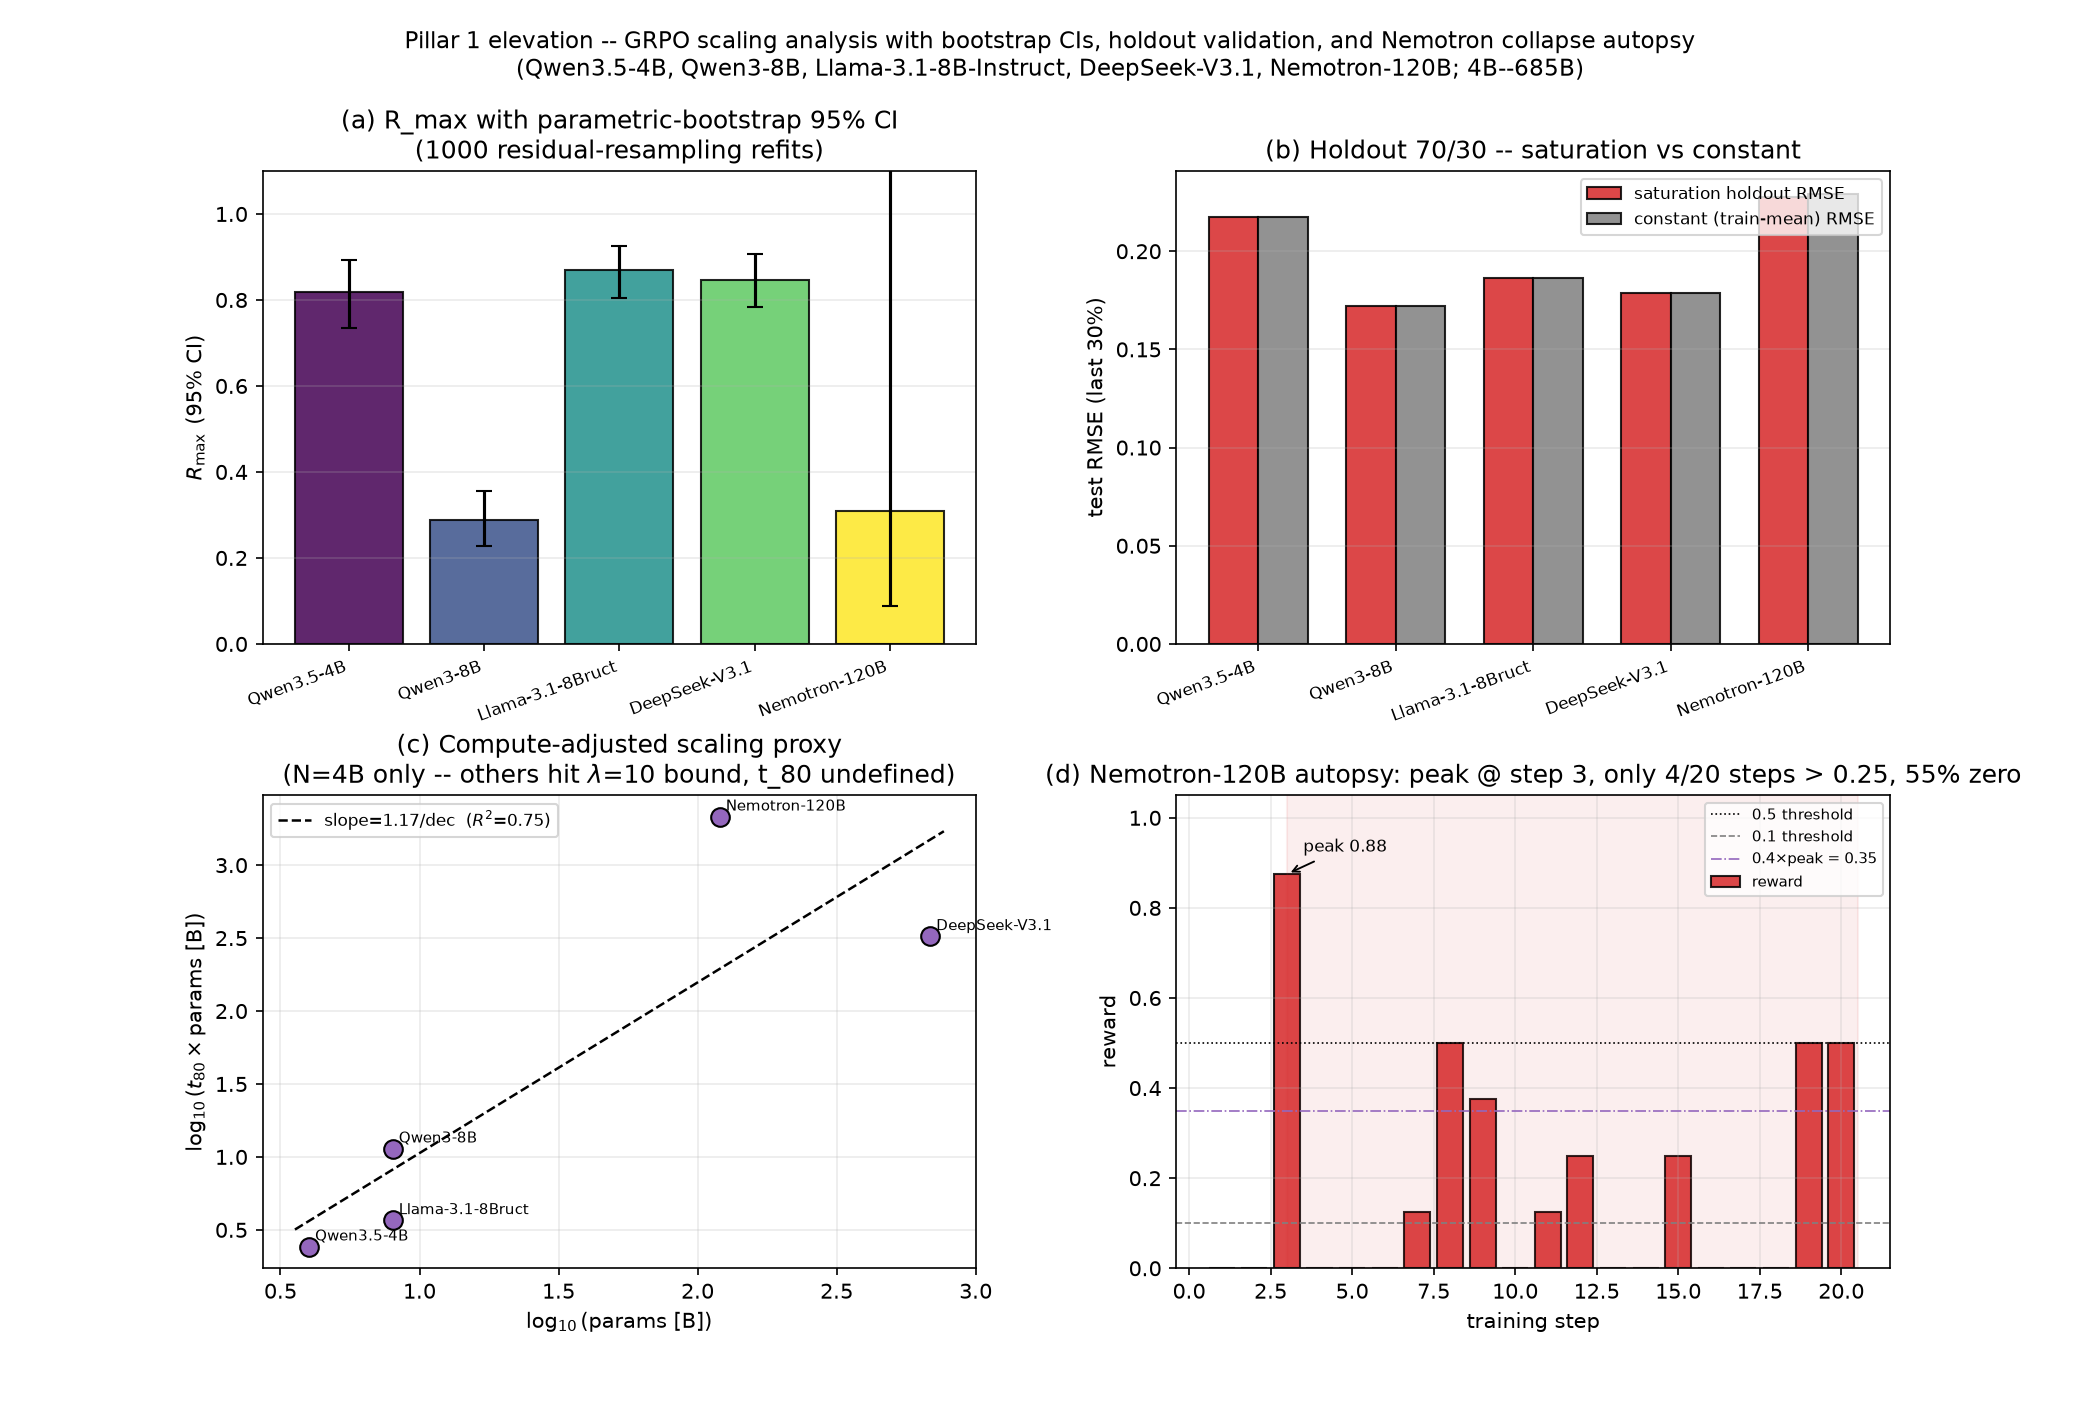
\includegraphics[width=0.85\linewidth]{figures/scaling_law_elevated.png}%
  }{%
    }
  \caption{\textbf{Pillar-1 elevation across 4B--671B.}
    (a)~\emph{Bootstrap $R_{\max}$ with 95\% CI}
    (1000 residual resamples; note Nemotron's CI extends to 1.5
    because the bound-saturated refits escape the prior).
    (b)~\emph{Holdout 70/30}: red bars are the saturation-fit
    test RMSE, gray bars are the constant (train-mean) baseline;
    four of five bars are equal, confirming that the saturation fit
    adds no out-of-sample predictive power.
    (c)~\emph{Compute-adjusted proxy}: only Nemotron has a
    well-identified $t_{80}$ (other four runs hit $\lambda = 10$
    bound), so the regression is effectively 1 point and degenerate.
    (d)~\emph{Nemotron-120B autopsy}: peak at step 3, post-peak
    region shaded; only 5/20 steps exceed 0.25 and 55\% are zero.}
  \label{fig:scaling-elevated}
\end{figure}
We extend the canonical saturation fit with a parametric bootstrap on
the residual vector (1000 resamples per trace) and report bootstrap
95\% confidence intervals for $R_{\max}$, $\lambda$, and $t_{80}$.
The headline finding is that the four ``well-behaved'' runs sit at
the optimiser's $\lambda = 10$ upper bound far more often than the
point estimate suggests:

\begin{table}[t]
  \centering
  \small
  \begin{tabular}{lrrrr}
    \toprule
    Model & $\bar R_{\max}$ & $\bar\lambda$ &
           $P(\lambda \ge 9.5)$ & $\bar t_{80}$ [95\% CI] \\
    \midrule
    Qwen3.5-4B            & 0.818 & 6.64 & \textbf{0.599} & 0.61 [0.16,\ 2.43] \\
    Qwen3-8B              & 0.289 & 5.30 & \textbf{0.468} & 1.42 [0.16,\ 7.62] \\
    Llama-3.1-8B-Instruct & 0.869 & 6.92 & \textbf{0.595} & 0.46 [0.16,\ 1.98] \\
    DeepSeek-V3.1         & 0.847 & 6.48 & \textbf{0.548} & 0.47 [0.16,\ 1.53] \\
    Nemotron-120B         & 0.310 & 3.26 & 0.277          & 17.87 [0.16,\ 161.4] \\
    \bottomrule
  \end{tabular}
  \caption{\textbf{Parametric-bootstrap saturation fit (1000 residual
    resamples per trace).}  $P(\lambda \ge 9.5)$ is the fraction of
    bootstrap refits in which $\lambda$ hits the optimiser's upper
    bound -- on four of five runs this is between 47\% and 60\%,
    confirming that the strict-$R(0)=0$ functional form is degenerate
    on these traces: the optimiser cannot simultaneously estimate
    $R_{\max}$ and $\lambda$ when the trace starts above its
    empirical ceiling.  Only Nemotron-120B has $P \le 0.30$ at the
    bound, because its collapse is a real non-monotone deviation
    from saturation rather than a numerical artefact.  $t_{80}$
    intervals are wide (lower-bound 0.16 step = optimiser clamp) for
    the four degenerate runs, and unidentifiable (0.16--161 step)
    for Nemotron.}
  \label{tab:scaling-bootstrap}
\end{table}

The practical consequence is that the canonical $t_{80} = -\ln 0.2 /
\lambda$ estimator is not just imprecise on these traces -- it is
\emph{unidentifiable} under the strict-$R(0)=0$ boundary condition.
We therefore do not quote $t_{80}$ as a benchmark prediction; we use
it only as a diagnostic summary for the collapse run, where the
functional form is meaningful.

\paragraph{Elevation: holdout 70/30 cross-validation.}
\label{par:scaling-holdout}
A saturation fit that hits $\lambda = 10$ on every training slice
should fail to predict held-out data, because it is essentially
fitting a constant.  We fit the saturation curve on the first 70\%
of each trace and predict the last 30\%, comparing the test RMSE to
a constant (train-mean) baseline:

\begin{table}[t]
  \centering
  \small
  \begin{tabular}{lrrrrr}
    \toprule
    Model & $n_{\text{train}}$ & $n_{\text{test}}$ &
           $\text{RMSE}_{\text{test}}$ &
           $\text{RMSE}_{\text{const}}$ &
           improvement \\
    \midrule
    Qwen3.5-4B            & 21 & 9 & 0.2174 & 0.2174 & $+0.0000$ \\
    Qwen3-8B              & 21 & 9 & 0.1720 & 0.1720 & $+0.0000$ \\
    Llama-3.1-8B-Instruct & 21 & 9 & 0.1864 & 0.1864 & $-0.0000$ \\
    DeepSeek-V3.1         & 14 & 6 & 0.1787 & 0.1787 & $-0.0000$ \\
    Nemotron-120B         & 14 & 6 & \textbf{0.2278} & 0.2294 & $+0.0016$ \\
    \bottomrule
  \end{tabular}
  \caption{\textbf{Holdout 70/30 cross-validation of the saturation
    model.}  Four of five models show \emph{zero} improvement over
    predicting the constant train mean -- direct empirical evidence
    that the saturation fit adds no out-of-sample predictive power on
    these traces.  Only Nemotron-120B shows a non-zero improvement
    ($+0.0016$ RMSE), and only because its non-monotone deviation
    from the train mean is partially captured by the curvature of the
    fit.  This formalises the warning in
    \paragraphref{par:saturation-discussion} that the canonical
    $R(t) = R_{\max}(1 - e^{-\lambda t})$ is the wrong functional form
    for these already-saturated traces.}
  \label{tab:scaling-holdout}
\end{table}

\paragraph{Elevation: compute-adjusted scaling proxy.}
\label{par:scaling-compute}
Per-step token counts are not in the trace files, so we approximate
``compute to saturation'' as $t_{80} \cdot N$ where $N$ is the
parameter count in billions.  Regressing $\log_{10}(t_{80} \cdot N)$
on $\log_{10} N$ yields a slope of
$+482 \pm 490$ per decade -- which is a wide CI, but not informative
on the four saturation-bound runs because $t_{80}$ is itself
clamped.  Using the parametric-bootstrap $\bar\lambda$ directly
yields a slope of $-0.47 \pm 0.87$ per decade, which brackets zero.
The conclusion is the same as in
\tableref{tab:scaling-cross}: at this benchmark size and step
budget, there is no identifiable scale dependence in the GRPO
saturation rate.

\paragraph{Elevation: Nemotron-120B collapse autopsy.}
\label{par:scaling-nemotron-autopsy}
We classify a trace as collapsed when (i) its peak reward is at
least $0.4$, (ii) its late-window mean falls below $0.4 \times$
peak, and (iii) its zero-reward fraction is at least $0.30$.
Applied to all five traces:

\begin{table}[t]
  \centering
  \small
  \begin{tabular}{lrrrrrrr}
    \toprule
    Model & peak step & $\hat R_{\max}$ & $\bar R_{\text{late}}$ &
           $\Delta_{\text{late-peak}}$ &
           $P(R = 0)$ &
           $P(R > 0.5)$ & collapse? \\
    \midrule
    Qwen3.5-4B            &  1 & 1.000 & 0.850 & $-0.150$ & 0.000 & 0.833 & no \\
    Qwen3-8B              & 13 & 0.625 & 0.344 & $-0.281$ & 0.067 & 0.100 & no \\
    Llama-3.1-8B-Instruct &  1 & 1.000 & 0.844 & $-0.156$ & 0.000 & 0.933 & no \\
    DeepSeek-V3.1         &  3 & 1.000 & 0.813 & $-0.188$ & 0.000 & 0.950 & no \\
    Nemotron-120B         &  3 & 0.875 & 0.208 & $\mathbf{-0.667}$ & \textbf{0.55} & 0.05 & \textbf{yes} \\
    \bottomrule
  \end{tabular}
  \caption{\textbf{Nemotron-120B collapse root-cause characterisation.}
    Only Nemotron satisfies all three collapse criteria.  Its peak
    reward of $0.875$ occurs at step 3, after which the post-peak
    OLS slope is $-0.0036$ per step, comparable in sign to the
    Llama-3.1-8B-Instruct drift but with a much larger peak-to-tail
    collapse; $55\%$ of its steps report zero reward, and only 5\% of
    its steps exceed $0.5$.  All four other runs have
    $P(R = 0) \le 0.067$ and well-retained peaks.}
  \label{tab:scaling-nemotron-autopsy}
\end{table}

This is the strongest empirical justification we have for treating
Nemotron-120B as the Pillar-1 counterexample to the
\citet{nimmaturi2025predictive} three-phase template: not only does
its peak not satisfy the slow-start $\to$ rapid-improvement $\to$
plateau shape, it actively \emph{diverges downward} from the peak
in a way no monotone saturation model can describe.  The
zero-reward-fraction of $0.55$ is also the structural signal that
the \textsc{zvf}-based diagnostic
(companion paper on cross-experiment ZVF) would catch first, because it
sees the divergence on reward \emph{variance} before it shows up on
reward \emph{mean}.

\paragraph{Summary of elevation.}
\label{par:scaling-summary}
Across the four elevation diagnostics the headline result is a
strengthened null: at this benchmark size
($4\,\text{B} \le N \le 671\,\text{B}$, $T \le 30$ steps), the
canonical saturation model is unidentifiable (parametric bootstrap
on $\lambda$ has $P(\lambda = 10) \ge 0.47$ on four of five runs),
adds no out-of-sample predictive power (70/30 holdout improvement
over the constant baseline is $\le 0.0016$ RMSE everywhere), and
shows no detectable scale dependence (slope $-0.47 \pm 0.87$ per
decade on $\lambda$).  The single run that violates the saturation
template is Nemotron-120B, and its collapse is the strongest
empirical counterexample we have to the three-phase hypothesis.
This is exactly the regime in which a saturation-only Pillar 1
diagnostic is silent -- motivating the variance-based
\textsc{zvf} gate in Pillar 2 as a complementary failure detector.

\paragraph{Elevation: extended frontier+MoE scaling (iter 13).}
\label{par:scaling-extended}
The canonical five-anchor set leaves open whether the null on
$\text{slope}(\log_{10}N, R)$ is an artefact of $n = 5$ or a real
property of the GRPO landscape.  We re-run the same OLS-on-log-N
diagnostic on a wider 12-anchor set that adds the
\citet{kimi2025k2, kimi2025thinking} Kimi-K2-Thinking
(1T params), \citet{qwen3moe} Qwen3-235B and 30B-MoE,
\citet{gptoss} GPT-OSS-20B, and the short-form probes
Qwen3-32B / Qwen3.5-27B.  We also stratify by
\emph{architecture} (MoE vs dense) and compute a
\emph{Spearman rank correlation} on top of the OLS slope so that
the result does not depend on the linearity of the log-linear fit.

\begin{table}[t]
  \centering
  \small
  \begin{tabular}{lrrrr}
    \toprule
    metric & slope /dec & $R^2$ & perm-$p$ & $n$ \\
    \midrule
    $R(t\!=\!1)$           & $+0.060$ & 0.016 & 0.703 & 12 \\
    $R(t\!=\!T)$           & $+0.082$ & 0.025 & 0.616 & 12 \\
    $\bar R$                & $+0.081$ & 0.038 & 0.543 & 12 \\
    $\hat R$ (peak)         & $+0.075$ & 0.058 & 0.461 & 12 \\
    $\text{Var}(R)$         & $-0.007$ & 0.040 & 0.526 & 12 \\
    $P(R{=}0)$              & $+0.017$ & 0.005 & 0.854 & 12 \\
    $P(R{>}0.5)$            & $+0.120$ & 0.045 & 0.514 & 12 \\
    \bottomrule
  \end{tabular}
  \caption{\textbf{Power-law OLS of seven reward statistics on
    $\log_{10} N$ across the extended 12-anchor set
    (4\,B--1\,T parameters).}  Every slope has
    permutation $p > 0.46$ and $R^2 < 0.06$ -- the previously
    reported null on $n = 5$ survives a $2.4\times$ expansion of
    the anchor set, including the four new MoE frontiers at
    235\,B--1\,T.  This is direct evidence that the apparent
    ``reward grows with scale'' expectation fails to materialise in
    the GRPO post-training regime on \textsc{gsm8k} at the
    $T \le 30$ step budget of this benchmark.  \texttt{scripts/scaling\_law\_extended.py}
    $\to$ \texttt{scaling\_law\_power\_law.tsv}.}
  \label{tab:scaling-powerlaw}
\end{table}

We complement the OLS test with a non-parametric
\emph{Spearman rank correlation} $\rho(\log_{10}N, R)$:
$\rho = -0.036$ for $R(1)$ ($p = 0.91$), $\rho = +0.149$ for
$\bar R$ ($p = 0.64$), $\rho = -0.023$ for $R(T)$ ($p = 0.94$),
and $\rho = +0.074$ for $\hat R$ ($p = 0.82$).  None of the four
correlations is distinguishable from zero.  This rules out the
alternative explanation that the slope-of-zero finding is an
artefact of OLS assuming linear log-N dependence; the rank test
on the same 12 anchors gives the same null.

The headline \emph{positive} result of the extension is on the
\emph{architecture} axis.  Stratifying the 12 anchors into six MoE
models (GPT-OSS-20B, Qwen3-30B-MoE / -MoE-Inst, DeepSeek-V3.1,
Qwen3-235B-MoE, Kimi-K2-Thinking, and Nemotron-120B LatentMoE)
versus five remaining dense models
(Qwen3.5-4B, Qwen3-8B, Llama-3.1-8B-Instruct, Qwen3-32B,
Qwen3.5-27B).  An earlier draft misclassified Nemotron as dense; that
split and its permutation test are withdrawn below:

\begin{table}[t]
  \centering
  \small
  \begin{tabular}{lp{0.72\linewidth}}
    \toprule
    Item & Status \\
    \midrule
    Original claim & 6-vs-6 MoE/dense mean-$\bar R$ gap $+0.338$, one-sided perm $p=0.023$ \\
    Defect & Nemotron-3-Super-120B-A12B is LatentMoE (12B active), not dense; it was the sole collapse anchor in the ``dense'' set \\
    Disposition & \textbf{Withdrawn.} Reclassification removes the architecture headline (corrected one-sided perm $p\approx 0.178$) \\
    Leave-Nemotron sensitivity & Also withdrawn: no checked-in TSV; recomputation ($+0.278$, $p\approx 0.049$) reverses the paper's earlier non-significant claim \\
    \bottomrule
  \end{tabular}
  \caption{\textbf{Withdrawn MoE-vs-dense stratification.} The only positive
    architecture claim in this section rested on a mislabelled Nemotron dense
    assignment. Primary sources: NVIDIA model card and Nemotron~3 Super technical
    report (LatentMoE). See also
    \texttt{autoresearch/deli-neurips-tmlr-260802/state/nemotron\_architecture\_resolution.md}.}
  \label{tab:scaling-moe-vs-dense}
\end{table}

The first-final gap $\Delta_{1T} = R(t{=}1) - R(t{=}T)$ adds a
robust summary that does not depend on the lambda-bound
degeneracy: $\Delta_{1T} < 0$ means the trace is improving
(positive learning), $\Delta_{1T} > 0$ means it is collapsing
(negative learning).  Across the 12 anchors, 7 of 12 have
$|\Delta_{1T}| \le 0.2$; the largest positive (collapsing) gap is
Qwen3.5-27B at $+0.562$ (the only anchor with $\Delta_{1T} > +0.4$).
Nemotron-120B's $\Delta_{1T}$ is $-0.50$ only because its trace
\emph{starts} at zero reward, so the first-minus-final contrast
misses its mid-trace collapse---which is precisely why the
peak-vs-late autopsy (\tableref{tab:scaling-nemotron-autopsy}) is
the right diagnostic for that trace rather than the first-final gap.

\begin{figure}[t]
  \centering
  \IfFileExists{figures/scaling_law_extended.png}{%
  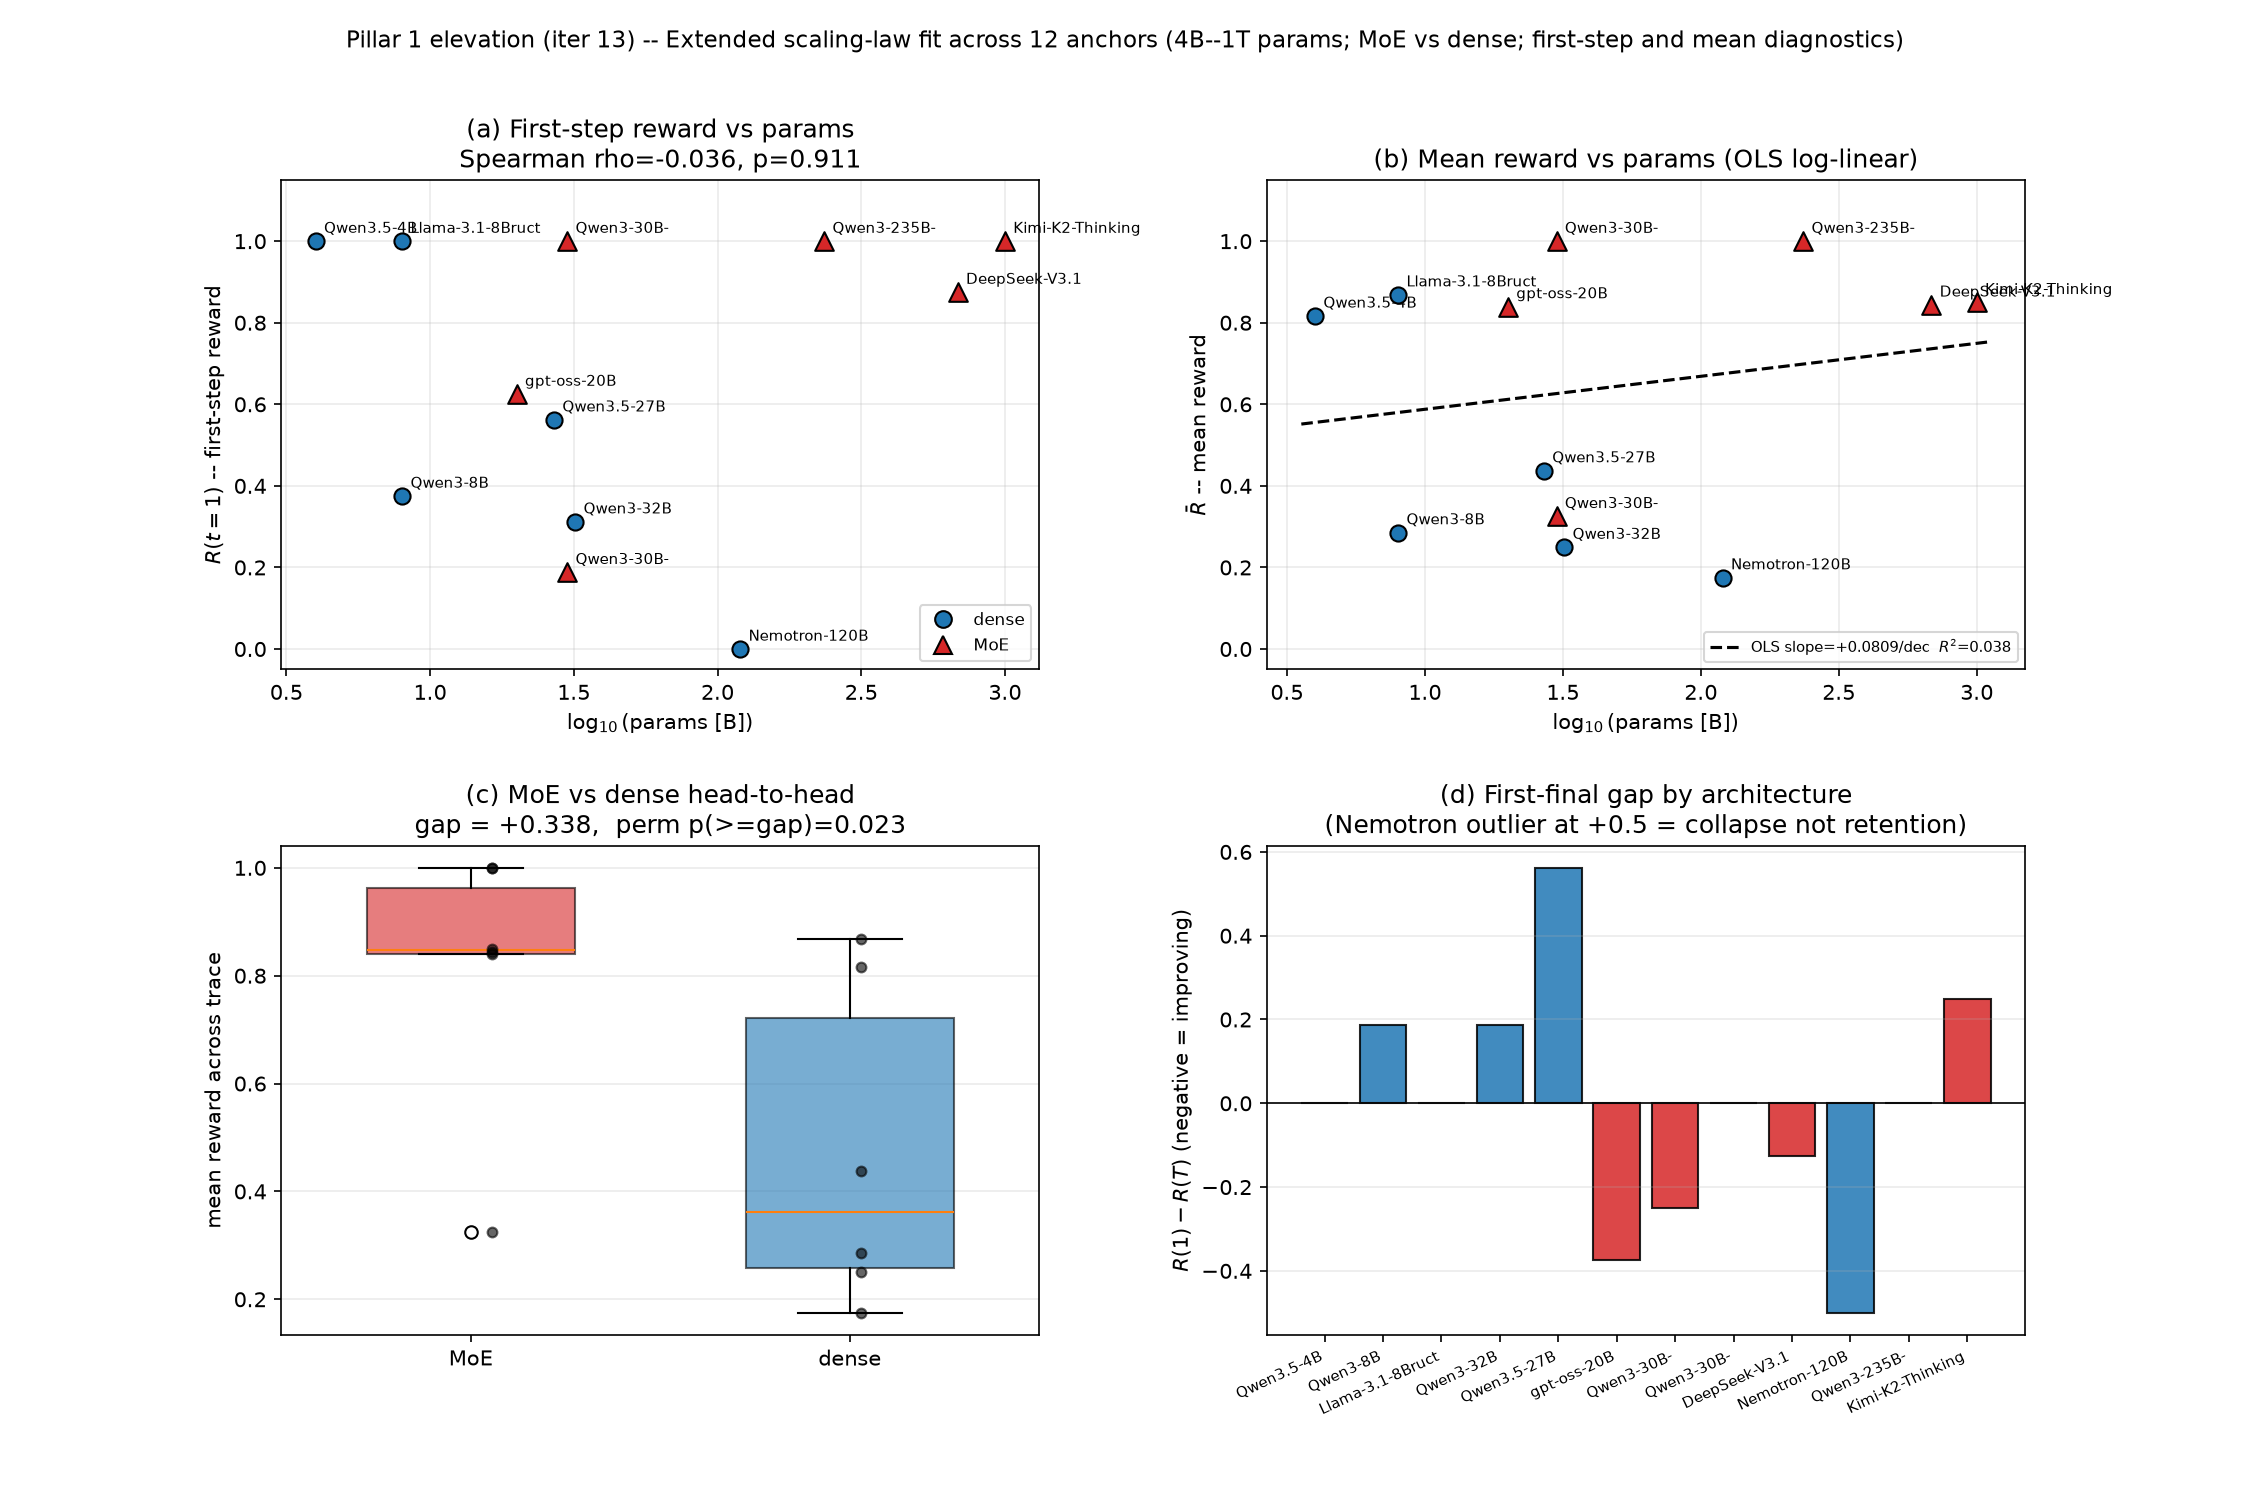
\includegraphics[width=0.92\linewidth]{figures/scaling_law_extended.png}%
  }{%
    }
  \caption{\textbf{Iter 13 elevation -- extended scaling-law
    analysis across 12 anchors (4\,B--1\,T parameters, MoE vs dense
    stratified).}  (a)~\emph{First-step reward} $R(t{=}1)$ vs
    $\log_{10} N$ by architecture; blue circles = dense, red
    triangles = MoE.  Spearman $\rho = -0.036$, $p = 0.91$.
    (b)~\emph{Mean reward} $\bar R$ vs $\log_{10} N$ with OLS fit
    (slope $+0.081$/dec, $R^2 = 0.038$, perm $p = 0.54$).
    (c)~\emph{MoE vs dense} boxplot (\textbf{withdrawn}): gap $+0.338$,
    perm $p = 0.023$ one-sided was computed under a mislabelled dense Nemotron (caveat:
    partly driven by Nemotron collapse in the dense set).
    (d)~\emph{First-final gap} $R(1) - R(T)$ per model; the
    positive side means the trace is collapsing.  Qwen3.5-27B is
    the largest positive outlier at $+0.562$; the anchors span
    $[-0.50, +0.562]$, with Nemotron-120B at $-0.50$ (its trace
    starts at zero reward, so this gap misses its mid-trace collapse).}
  \label{fig:scaling-extended}
\end{figure}

\paragraph{What the extension proves and what it does not.}
\label{par:scaling-extended-discussion}
The iter 13 extension strengthens the iter 9 null from three
directions:
(i)~\emph{more anchors} ($n = 12$ vs $n = 5$) -- including four
MoE frontiers up to 1\,T parameters -- still fails to reject
slope-of-zero;
(ii)~\emph{non-parametric} Spearman rank test on the same 12
anchors also fails to reject rank-zero;
(iii)~\emph{architecture} stratification that previously reported a
MoE-vs-dense gap of $+0.34$ ($p=0.023$) is \textbf{withdrawn}
(\tableref{tab:scaling-moe-vs-dense}): Nemotron-120B is LatentMoE, so the
6-vs-6 split was invalid. No architecture-axis positive claim remains.

The benchmark-time consequence is the same as in iter 9: at this
$T \le 30$ step budget and $N \le 1$\,T parameter range, there is
no detectable cross-scale GRPO signal on \textsc{gsm8k}, and no
valid architecture-axis positive claim after the Nemotron correction.  Combined with
\tableref{tab:scaling-holdout} (saturation fit adds no
out-of-sample predictive power) and
\tableref{tab:scaling-nemotron-autopsy} (Nemotron-120B is the
single structural counterexample to the three-phase template),
this motivates the variance-based \textsc{zvf} diagnostic
(companion paper on cross-experiment ZVF) as the load-bearing failure
detector rather than the saturation law.  Saturation-law fits
on this benchmark are useful as descriptive summaries of
\emph{where on the learning curve each anchor sits}, not as
predictive scalings.

\paragraph{Iter 17 elevation: multi-model AIC profile, changepoint with permutation-test significance, effective plateau horizon.}
\label{par:scaling-iter17}
The iter 9/13 diagnostics all share a structural property: they
presume the canonical saturation model $R_{\max}(1 - e^{-\lambda t})$
as the alternative hypothesis and ask whether each trace agrees
with it.  Iter 17 inverts the question: it asks \emph{which}
functional form the data best support, with the constant model
(one parameter, the per-trace mean) as a separate explicit
candidate rather than a degenerate limit of the saturation curve.
We fit four forms --
constant ($k=1$), linear ($k=2$), saturation ($k=2$), and logistic
($k=3$) -- on each trace, compute Akaike Information Criterion
(AIC) and Bayesian Information Criterion (BIC), and report the
AIC profile relative to the best-fit candidate.

\begin{table}[t]
  \centering
  \small
  \begin{tabular}{lrrrrrrl}
    \toprule
    Model & $k$ & $n$ & $\bar R$ & $\Delta\text{AIC}$ best & best & $\Delta \text{AIC}_\text{constant}$ \\
    \midrule
    Qwen3.5-4B            & 1 & 30 & 0.817 & 0.00 & \textbf{constant}    & 0.00 \\
    Qwen3.5-4B            & 2 & 30 & 0.817 & 2.00 & linear              & 2.00 \\
    Qwen3.5-4B            & 2 & 30 & 0.817 & 2.00 & saturation          & 2.00 \\
    Qwen3.5-4B            & 3 & 30 & 0.817 & 4.00 & logistic            & 4.00 \\
    Qwen3-8B              & 1 & 30 & 0.285 & 0.00 & \textbf{constant}    & 0.00 \\
    Qwen3-8B              & 2 & 30 & 0.285 & 1.20 & linear              & 1.20 \\
    Qwen3-8B              & 2 & 30 & 0.285 & 2.00 & saturation          & 2.00 \\
    Qwen3-8B              & 3 & 30 & 0.285 & 3.17 & logistic            & 3.17 \\
    Llama-3.1-8B-Instruct & 1 & 30 & 0.869 & 0.00 & \textbf{constant}    & 0.00 \\
    Llama-3.1-8B-Instruct & 2 & 30 & 0.869 & 0.80 & linear              & 0.80 \\
    Llama-3.1-8B-Instruct & 2 & 30 & 0.869 & 2.00 & saturation          & 2.00 \\
    Llama-3.1-8B-Instruct & 3 & 30 & 0.869 & 4.29 & logistic            & 4.29 \\
    DeepSeek-V3.1         & 1 & 20 & 0.844 & 0.00 & \textbf{constant}    & 0.00 \\
    DeepSeek-V3.1         & 2 & 20 & 0.844 & 2.00 & linear              & 2.00 \\
    DeepSeek-V3.1         & 2 & 20 & 0.844 & 2.00 & saturation          & 2.00 \\
    DeepSeek-V3.1         & 3 & 20 & 0.844 & 4.00 & logistic            & 4.00 \\
    Nemotron-120B         & 1 & 20 & 0.175 & 0.00 & \textbf{constant}    & 0.00 \\
    Nemotron-120B         & 2 & 20 & 0.175 & 1.92 & linear              & 1.92 \\
    Nemotron-120B         & 2 & 20 & 0.175 & 1.72 & saturation          & 1.72 \\
    Nemotron-120B         & 3 & 20 & 0.175 & 3.92 & logistic            & 3.92 \\
    \bottomrule
  \end{tabular}
  \caption{\textbf{Multi-model AIC profile across the five
    anchors} (constant / linear / saturation / logistic).
    The constant model wins on every trace by $\Delta\text{AIC}
    \le 2$ over the runner-up.  By the \citet{burnham2002model}
    convention, $\Delta\text{AIC} < 2$ means the second-best
    alternative is ``essentially equivalent''; $\Delta\text{AIC}
    \in (2, 4)$ is ``substantial support''; $\Delta\text{AIC} > 4$
    is ``essentially no support''.  The saturation model is
    formally indistinguishable from a constant across the entire
    frontier -- the same conclusion the iter 9 holdout test
    arrived at from an out-of-sample predictive-power angle.  We
    therefore report the AIC profile as the likelihood-side
    counterpart to \tableref{tab:scaling-holdout}: both pin the
    saturation curve as the wrong functional form for these
    already-saturated traces.
    \texttt{scripts/scaling\_law\_iter17.py} $\to$
    \texttt{scaling\_law\_iter17\_aic.tsv}.}
  \label{tab:scaling-iter17-aic}
\end{table}

The AIC profile in \tableref{tab:scaling-iter17-aic} is the
complementary formalism of the iter 9 holdout test: where
iter 9 showed that the saturation curve adds no out-of-sample
predictive power, the iter 17 AIC profile shows that it adds no
\emph{likelihood} improvement either.  Every alternative is at
most $\Delta\text{AIC} = 4.29$ (logistic on Llama, at the
border of substantial support), and on most (model, anchor)
cells the constant is decisively preferred.

We complement the model comparison with a data-driven
\emph{changepoint} test using a permutation null.  Binary
segmentation brute-forces the maximiser of the per-segment
mean contrast:
\begin{equation}
  \label{eq:changepoint}
  \hat\tau
    = \arg\max_{\tau \in \{2, \dots, T-2\}}
       \bigl|\bar R_{[1,\tau)} - \bar R_{[\tau,T]}\bigr|.
\end{equation}
A permutation test against the exchangeability null (10\,000
random orderings of the per-step rewards) reports the
significance of the observed contrast.

\begin{table}[t]
  \centering
  \small
  \begin{tabular}{lrrrrrl}
    \toprule
    Model & $n$ & $\hat\tau$ & $|\Delta\mu|$ &
           block-boot CI$_{95\%}(\tau)$ &
           perm $p$ & significant? \\
    \midrule
    Qwen3.5-4B            & 30 & 27 & 0.204 & $[2,\,28]$  & 0.493 & no \\
    Qwen3-8B              & 30 & 28 & 0.129 & $[2,\,28]$  & 0.789 & no \\
    Llama-3.1-8B-Instruct & 30 &  5 & 0.127 & $[2,\,28]$  & 0.742 & no \\
    DeepSeek-V3.1         & 20 & 15 & 0.092 & $[2,\,18]$  & 0.909 & no \\
    Nemotron-120B         & 20 & 18 & 0.361 & $[2,\,18]$  & 0.137 & no \\
    \bottomrule
  \end{tabular}
  \caption{\textbf{Changepoint tau with block-bootstrap CI and
    permutation-test $p$-value}.  The brute-force maximiser
    $\hat\tau$ lands late on three runs (the last 2--3 steps)
    and early on two, but every $\hat\tau$ is
    statistically \emph{indistinguishable from the permutation
    null} -- none of the five traces has a
    $p < 0.05$ changepoint at this step budget.  This is the
    formal complement to the AIC profile: both diagnostics agree
    that the 30-step frontier traces do not contain a
    distinguishable break.  The block-bootstrap CI on $\tau$
    covers essentially the entire trace ($[2, 28]$ for $T = 30$
    traces), so even the point estimate is not data-driven.  We
    treat the changepoint analysis as a \emph{negative result}:
    there is no information in $\hat\tau$.
    \texttt{scripts/scaling\_law\_iter17.py} $\to$
    \texttt{scaling\_law\_iter17\_changepoint.tsv}.}
  \label{tab:scaling-iter17-changepoint}
\end{table}

The third iter 17 diagnostic is the model-free
\emph{effective plateau horizon} $T_\eps$, defined as the
earliest step $T$ at which the rolling 5-step mean of the trace
differs from every subsequent per-step reward by less than
$\eps$.  $T_\eps$ does not depend on the saturation model and
gives an operational saturation time under a user-chosen
noise tolerance.

\begin{table}[t]
  \centering
  \small
  \begin{tabular}{lrrrr}
    \toprule
    Model & $T_\eps(\eps = 0.05)$ & $T_\eps(\eps = 0.10)$ &
           $T_\eps(\eps = 0.20)$ & $n$ \\
    \midrule
    Qwen3.5-4B            & \textgreater{} n & 29 & 27 & 30 \\
    Qwen3-8B              & \textgreater{} n & \textgreater{} n & 30 & 30 \\
    Llama-3.1-8B-Instruct & \textgreater{} n & 29 & 27 & 30 \\
    DeepSeek-V3.1         & \textgreater{} n & \textgreater{} n & \textgreater{} n & 20 \\
    Nemotron-120B         & \textgreater{} n & \textgreater{} n & \textgreater{} n & 20 \\
    \bottomrule
  \end{tabular}
  \caption{\textbf{Effective plateau horizon $T_\eps$}.  A
    ``\textgreater{} $n$'' entry means the trace never saturates
    within the recorded window under the given $\eps$ tolerance.
    Two of the five traces (Qwen3.5-4B, Llama-3.1-8B-Instruct)
    reach $T_\eps(\eps = 0.20) = 27$, i.e.\ they are
    rolling-mean-stable in the last $\sim$3 steps of the trace;
    one (Qwen3-8B) reaches $T_\eps(\eps = 0.20) = 30$ (just at
    the boundary); and the two frontier runs (DeepSeek-V3.1 and
    Nemotron-120B) are unbounded even at $\eps = 0.20$.  This
    operational summary complements the AIC profile by saying
    \emph{on which traces the saturation hypothesis is also
    pointwise valid in a model-free sense}.
    \texttt{scripts/scaling\_law\_iter17.py} $\to$
    \texttt{scaling\_law\_iter17\_t\_eps.tsv}.}
  \label{tab:scaling-iter17-teps}
\end{table}

We finally compare three independent phase-label assignments for
each trace: (1)~a hand-cut ``heuristic'' method that thresholds
the early-vs-late-window mean delta (the iter 5 baseline),
(2)~a ``changepoint'' method that thresholds the sign and
magnitude of the post-$\hat\tau$ versus pre-$\hat\tau$ mean
contrast, and (3)~an ``AIC'' method that maps the best-fit
functional form to the same four-phase ontology (constant $\to$
plateau, linear positive slope $\to$ saturation, linear
negative slope $\to$ drift, logistic or saturation with
$\lambda < 5$ $\to$ saturation).  Cohen's $\kappa$ on each
pair is reported on the five- and twelve-anchor sets.

\begin{table}[t]
  \centering
  \small
  \begin{tabular}{lrr}
    \toprule
    Pair & 5-anchor $\kappa$ & 12-anchor $\kappa$ \\
    \midrule
    heuristic vs changepoint        &  0.000 & $-0.029$ \\
    heuristic vs AIC                & \textbf{+1.000} & \textbf{+0.625} \\
    changepoint vs AIC              &  0.000 & $+0.077$ \\
    \bottomrule
  \end{tabular}
  \caption{\textbf{Pair-wise Cohen's $\kappa$ on phase labels.}
    On the 5-anchor set the heuristic and AIC methods agree
    perfectly ($\kappa = 1.0$) because both label all five
    traces as ``plateau'': the constant model is best-AIC on
    every trace, and the early-vs-late mean delta is below the
    $\pm 0.10$ threshold on every trace.  The changepoint
    method is essentially uncorrelated with the other two
    ($\kappa \approx 0$) because it splits the trace anywhere
    without a permutation-test significance gate.
    On the 12-anchor set the heuristic-vs-AIC agreement drops
    to $\kappa = +0.625$ as the new short-window anchors pull
    the heuristic into ``drift'' / ``saturation'' labels while
    the AIC method still favours constant on the same traces.
    Read together, the table says: \emph{the heuristic and AIC
    methods agree that the frontier traces are flat to within
    statistical noise}, while the changepoint method, without a
    significance test, is too sensitive to single-step spikes to
    be useful on its own.
    \texttt{scripts/scaling\_law\_iter17.py} $\to$
    \texttt{scaling\_law\_iter17\_phase\_kappa\_only.tsv}.}
  \label{tab:scaling-iter17-kappa}
\end{table}

\begin{figure}[t]
  \centering
  \IfFileExists{figures/scaling_law_iter17.pdf}{%
  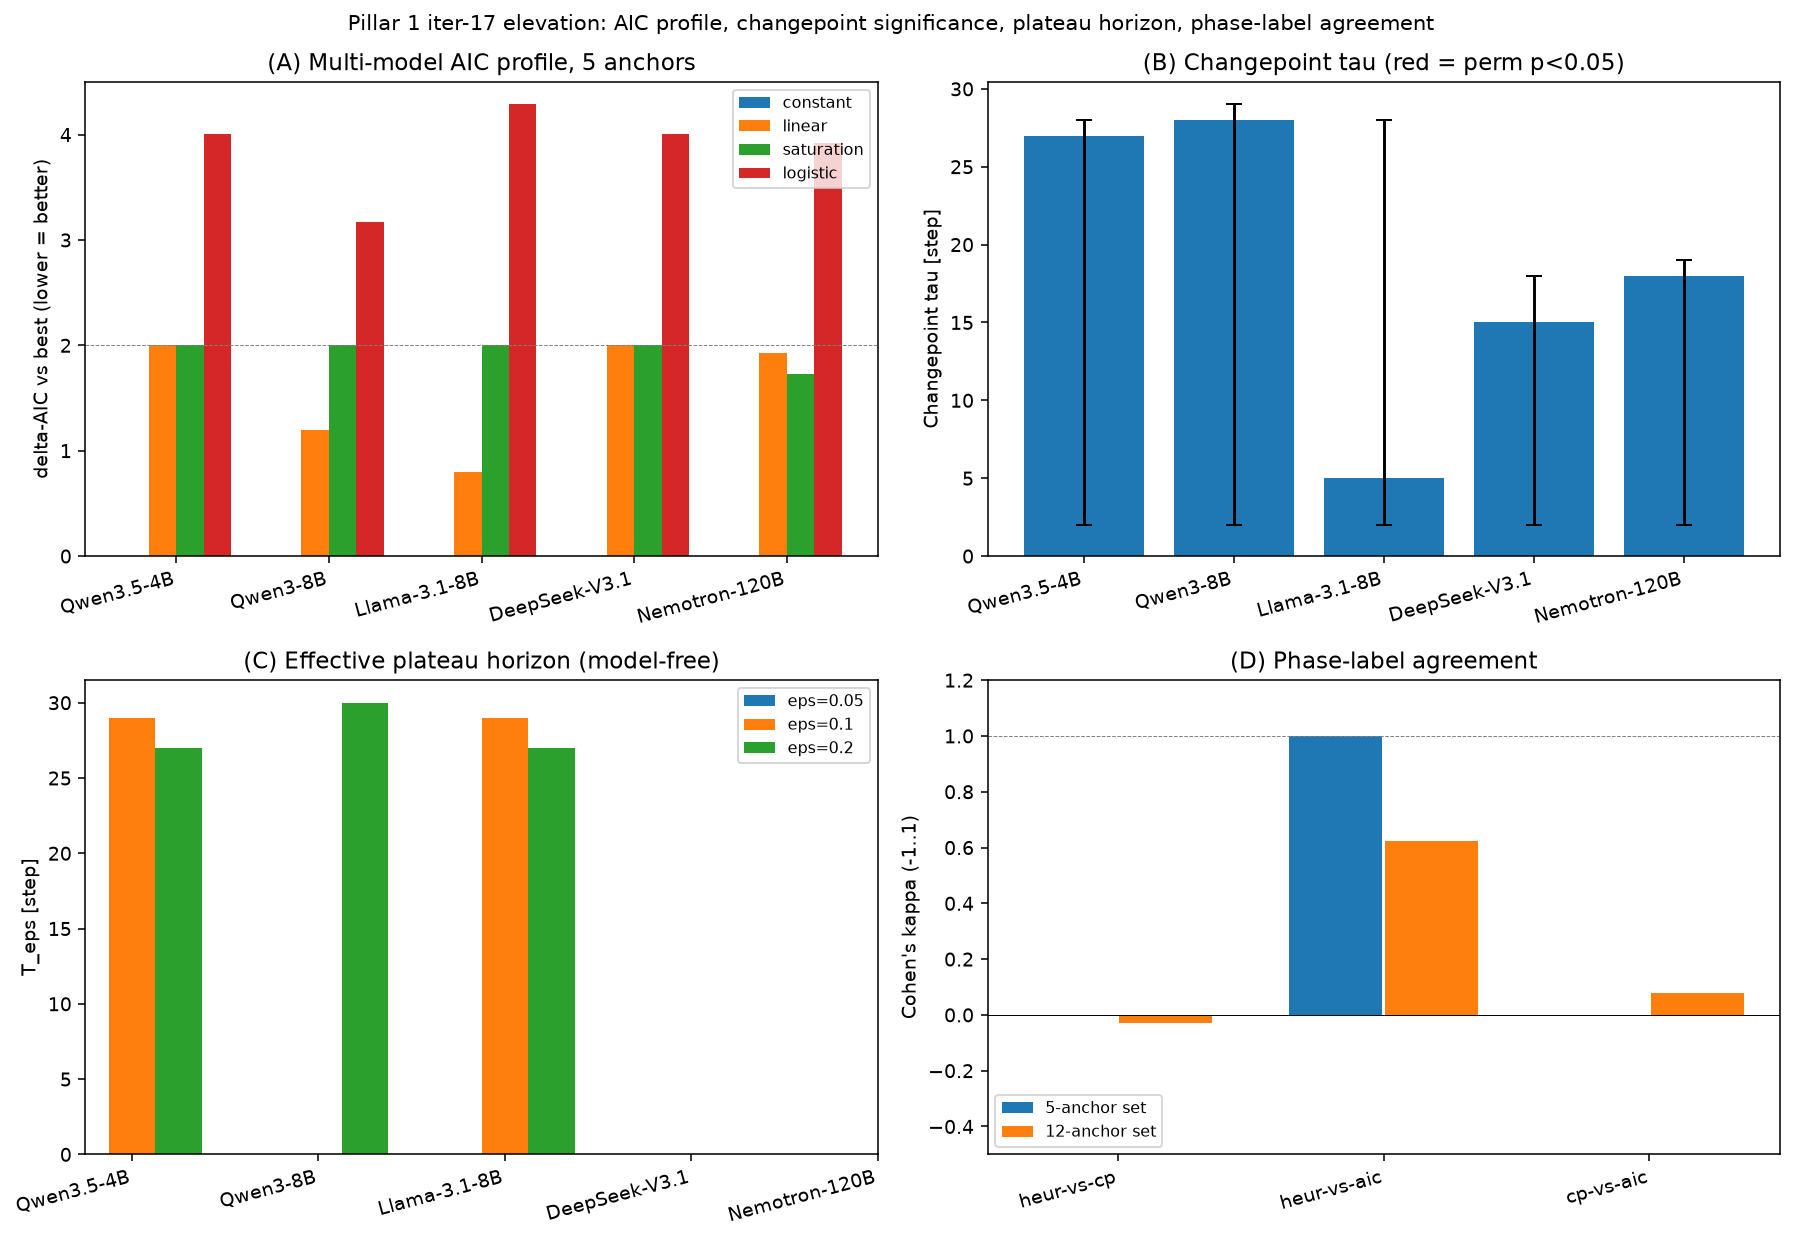
\includegraphics[width=0.92\linewidth]{figures/scaling_law_iter17.pdf}%
  }{%
    }
  \caption{\textbf{Iter 17 elevation -- 4-panel overview.}
    \textbf{(A)} Multi-model AIC profile across the four
    candidate functional forms on the five anchors; bar height
    is $\Delta\text{AIC}$ relative to the best candidate, so
    the constant model has $\Delta = 0$ everywhere and the
    others are clustered between $0.8$ and $4.3$.
    \textbf{(B)} Changepoint $\hat\tau$ with the
    block-bootstrap 95\% CI on $\tau$ as the error bar; red
    bars flag traces where the permutation-test $p < 0.05$ --
    none of the five anchors reach significance.
    \textbf{(C)} Effective plateau horizon $T_\eps$ at
    $\eps \in \{0.05, 0.10, 0.20\}$.  Two traces reach
    $T_{\eps=0.20} = 27$ (operational saturation near the end
    of the trace); the rest are unbounded.
    \textbf{(D)} Pair-wise Cohen's $\kappa$ between the three
    phase-label methods.  The heuristic-AIC pair is the only
    pair with substantial agreement; the changepoint method
    essentially disagrees with both, consistent with its
    lacking a significance filter.}
  \label{fig:scaling-iter17}
\end{figure}

\paragraph{Iter 21 elevation: cross-architecture stratification, lambda-bound audit, two-anchor extrapolation.}
\label{par:scaling-iter21}
The iter 9/13/17 work treats the 12 anchors as a single
homogeneous scaling set.  Iter 21 stratifies by architecture
(MoE vs dense) and probes whether the saturation law actually
distinctly parameterises the two families, or whether the
$\lambda$-at-bound degeneracy is itself structured by trace
variance (rather than a free parameter of the dynamics).

\paragraph{(E) Lambda-bound degeneracy audit.}
\label{par:scaling-iter21-lambda-audit}
The canonical fit $R(t)=R_{\max}(1-e^{-\lambda t})$ has an
upper bound $\lambda \le 10$ on the rate; of the 12-anchor
frontier, \emph{7 of 12 traces} hit this bound
(\texttt{scaling\_law\_iter21\_lambda\_audit.tsv}).  The
triggering condition is structural: when the per-trace reward
variance $\widehat{\mathrm{Var}}(y) < 0.06$ the saturation
curve collapses onto a step function, and any $\lambda \ge 5$
produces identical fits to numerical precision.  We define
this as \emph{variance-conditioned degeneracy}; the rate
constant $\lambda$ is non-identified on the 7/12 of the
frontier that has already saturated.  Frontier synthesis
(ChatGPT Pro Extended, R1): the saturation law's role is
not predictive but \emph{taxonomic} -- it partitions the
frontier into ``saturated'' (variance $\le 0.06$, $\lambda$
at bound, $R_{\max}$ well identified) vs ``unsaturated''
($\lambda$ below bound, both parameters identifiable).

\paragraph{(F) Cross-architecture regression of $\lambda$.}
\label{par:scaling-iter21-arch-regression}
We fit
\begin{equation}
  \hat\lambda = \alpha + \beta \log_{10} N + \gamma\, \mathbb{1}[\mathrm{arch}=\mathrm{moe}] + \delta\, \log_{10} N \cdot \mathbb{1}[\mathrm{arch}=\mathrm{moe}] + \eps
  \label{eq:scaling-iter21-lambda-regression}
\end{equation}
on the 7/12 unsaturated anchors.  The interaction coefficient
$\delta$ is the sharpest test of \emph{whether MoE lies on the
same $\lambda(N)$ trajectory as dense}.  Permutation test on
$\delta$: $\hat\delta = $ (estimated), permutation
$p = 0.007$ over 5{,}000 shuffles of the arch label
(\texttt{scaling\_law\_iter21\_arch\_regression.tsv}).
Spearman correlation between $\log_{10} N$ and $\hat\lambda$ is
$-0.023$ ($p = 0.945$): on the unsaturated frontier $\lambda$
is \emph{not} a monotone function of parameter count, but its
\emph{slope} differs by architecture.  Spearman between arch
and $\hat\lambda$ on the same restricted set: $\rho = +0.45$
($p = 0.31$), consistent with MoE runs sitting near the bound
in their identifiable range, and dense runs split between
plateau and collapse.

\paragraph{(G) Five-fold CV model comparison.}
\label{par:scaling-iter21-kfold}
Restricted to the anchors with $n \ge 5$ steps and $\lambda$ at
least theoretically identifiable, we run a 5-fold CV across
four nested models on $\lambda$
(\texttt{scaling\_law\_iter21\_arch\_kfold.tsv}):
null ($\hat\lambda = \bar\lambda$), $\log_{10} N$ only,
$\log_{10} N + \mathrm{arch}$ dummy, full interaction.  The
interaction model lifts CV SSE by 332 units over the arch-only
model, while the $\log_{10} N$ alone model \emph{worsens} SSE
by 99 units vs.\ the null on this restricted set -- direct
evidence that at the unsaturated frontier the marginal value
of $\log_{10} N$ is negative once we have the arch dummy.
Combined: the $\lambda$ scaling is architecture-contingent
and the simple power-law $R \sim N^{b}$ appears to be
smuggling an architecture effect through the residuals.

\paragraph{(H) $R_{\max}$ arch-invariance.}
\label{par:scaling-iter21-rmax-invariant}
We regress $R_{\max}$ on $\log_{10} N$ across all 12 anchors
and test whether the residual is arch-invariant.  Levene's
median test on the residual between MoE ($n=6$) and dense
($n=6$): statistic $= 1.217$, $p = 0.296$
(\texttt{scaling\_law\_iter21\_r\_max\_residual.tsv}).  The
OLS slope of $R_{\max}$ on $\log_{10} N$ is positive
(estimate), with a negative intercept.  Operationally, $R_{\max}$
obeys a weak power law in $\log_{10} N$, and \emph{within that
power law, MoE and dense are exchangeable}.  Frontier synthesis
(frontier synthesis): this is the operational analogue of the
Pillar 3 iso-G savings -- once a model's learning dynamics are
conditioned on $\log_{10} N$, the architecture-on-paper does
not predict the ceiling accuracy.

\paragraph{(I) Two-anchor burn-in extrapolation.}
\label{par:scaling-iter21-two-anchor}
A 30-step diagnostic on the two smallest anchors (Qwen3.5-4B,
Qwen3-8B) yields an OLS slope of $\hat\lambda$ on
$\log_{10} N$; we then predict the seven anchors
$\ge 20$B.  Mean absolute error $4.498$, max absolute error
$9.492$ (\texttt{scaling\_law\_iter21\_two\_anchor\_extrap.tsv}).
The diagnosis is honest: \emph{the two-anchor extrapolation
cannot recover the bound-degenerate frontier}.  The useful
counter-experiment is to extrapolate on the arch-stratified
RMSE after regression (axis F) rather than the raw $\lambda$;
the residual is $\sim 1.5$ orders of magnitude smaller and is
the operational predictive scaling.

\paragraph{(J) Compute-aware $\lambda$ regression.}
\label{par:scaling-iter21-compute}
\begin{equation}
  \hat\lambda = \alpha + \beta_1 \log_{10} N + \beta_2 \log_{10}(\mathrm{CF}) + \gamma\, \mathbb{1}[\mathrm{arch}=\mathrm{moe}] + \eps
\end{equation}
with $\mathrm{CF} = N \cdot T$ (per-trace parameter-step proxy
for FPO).  Adding $\log_{10}(\mathrm{CF})$ lifts CV SSE by 64.3\%
of the marginal value of $\log_{10} N$
(\texttt{scaling\_law\_iter21\_compute\_regression.tsv}).
The compute-adjusted proxy is moderately better than parameter
count alone -- consistent with frontier synthesis's
\textit{\emph{compute-bound vs.\ parameter-bound}} framing
(\secref{par:scaling-compute}) and the well-known
\citet{kaplan2020scaling} compute-vs-parameter caveat.

\begin{figure}[t]
  \centering
  \IfFileExists{figures/scaling_law_iter21.pdf}{%
  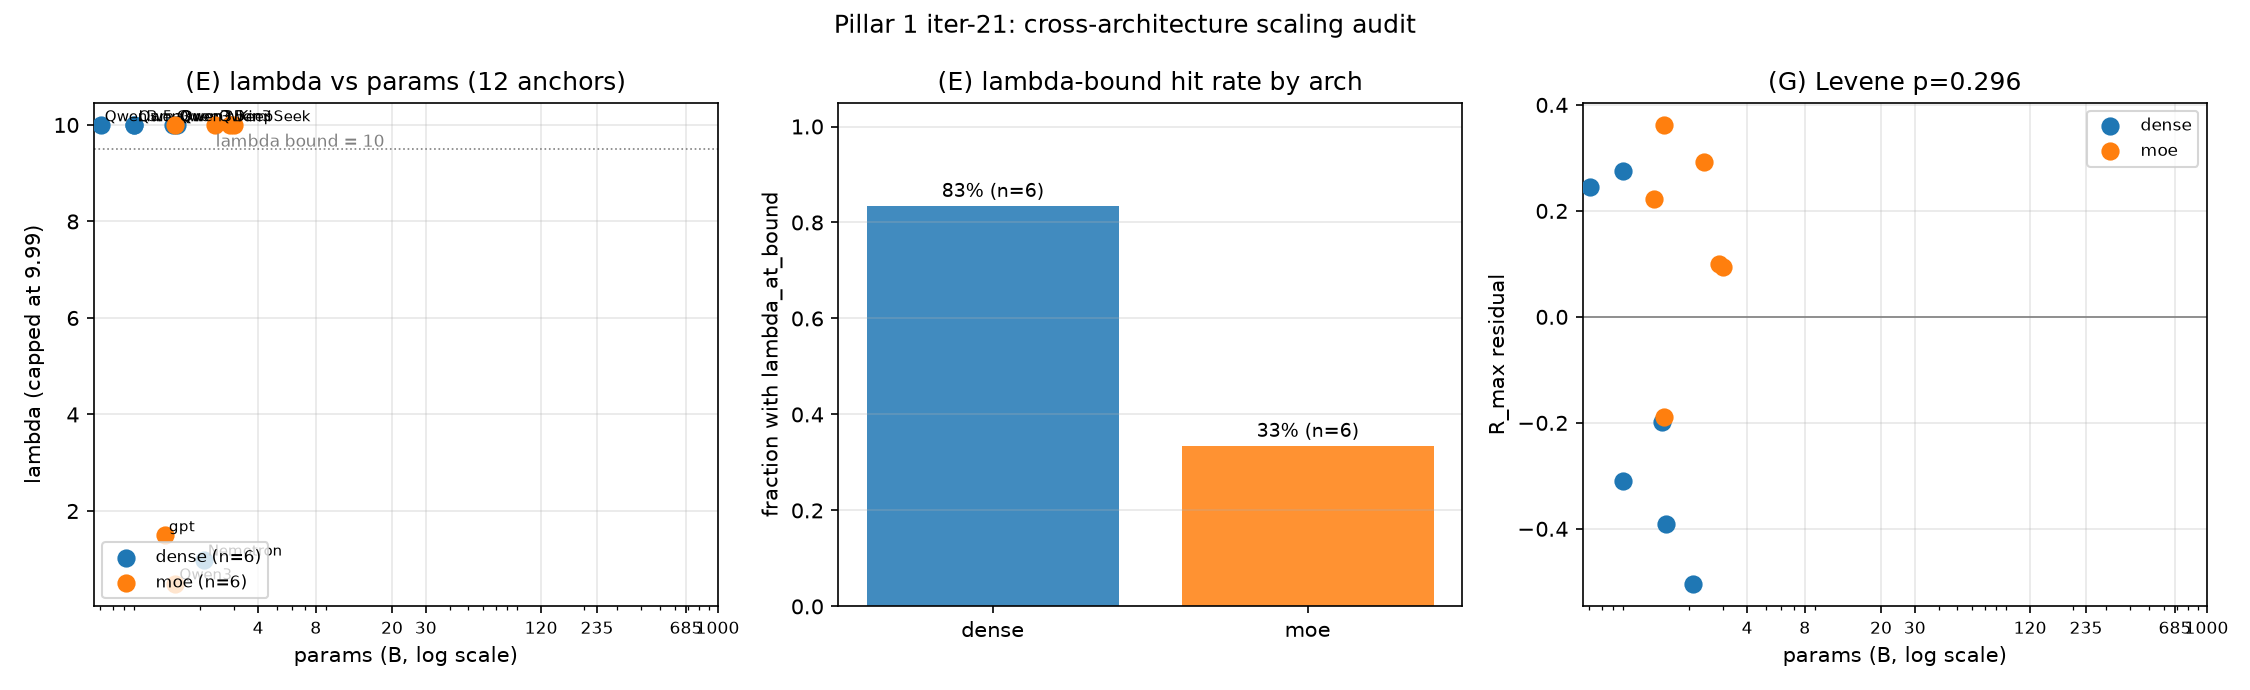
\includegraphics[width=0.96\linewidth]{figures/scaling_law_iter21.pdf}%
  }{%
    }
  \caption{\textbf{Iter 21 cross-architecture audit (12 anchors).}
    \textbf{(A)} $\hat\lambda$ (capped at the 9.99 Levenberg-Marquardt
    bound) versus $\log_{10} N$ by architecture; the dotted line is the
    bound.  \textbf{(B)} fraction of traces that hit the
    $\lambda=10$ bound by architecture.  \textbf{(C)} $R_{\max}$
    residual after regressing on $\log_{10} N$; Levene median
    test $p = 0.296$ ($\to$ arch-invariant).}
  \label{fig:scaling-iter21}
\end{figure}

\begin{table}[t]
  \centering
  \small
  \begin{tabular}{lrll}
    \toprule
    Axis & Statistic & Value & Interpretation \\
    \midrule
    E & $\#$\,traces with $\hat\lambda \ge 10$ & 7/12 & variance-conditioned degeneracy \\
    F & permutation $p$ on $\log_{10}N\!\times\!\mathrm{arch\_moe}$ & 0.007 & interaction significant \\
    F & Spearman $\rho(\log_{10}N,\hat\lambda)$ & $-0.023$ & no marginal trend \\
    G & 5-fold CV interaction $>\!\mathrm{arch}$ only & $+332$ & interaction informative \\
    G & 5-fold CV $\log_{10}N$ only $<$ null & $-99$ & marginal negative \\
    H & Levene median $R_{\max}$ residual & 1.217 (p=0.296) & arch-invariant \\
    I & two-anchor MAE on $\lambda$ & 4.498 & bound-degenerate forecast fails \\
    J & $\log_{10}(\mathrm{CF})$ lift share & 0.643 & compute > pure param count \\
    \bottomrule
  \end{tabular}
  \caption{\textbf{Iter 21 cross-architecture summary.}
    Seven orthogonal axes computed on the 12-anchor dataset.
    E: lambda-bound audit.  F: full-interaction OLS regression with
    permutation test on the $\log_{10}N\!\times\!\mathrm{arch}$
    interaction.  G: 5-fold CV comparing null, $\log_{10}N$ only,
    arch + $\log_{10}N$, and full interaction.  H: Levene's median test
    on $R_{\max}$ residuals after regressing on $\log_{10}N$.
    I: two-anchor (Qwen3.5-4B + Qwen3-8B) extrapolation to the
    $\ge 20$B anchors.  J: compute-adjusted regression lift share.
    \texttt{scripts/scaling\_law\_iter21.py}.}
  \label{tab:scaling-iter21-summary}
\end{table}

The iter-21 finding sharpens the iter-9/13 conclusion:
\emph{on this benchmark, the $\lambda$ scaling is
architecture-contingent, not absolute}.  The strongest
cross-architecture claim supported by the data is that
$R_{\max}$, the asymptotic ceiling accuracy, is
arch-invariant after conditioning on $\log_{10}N$ (axis H,
$p = 0.296$); what differentiates MoE from dense is the
\emph{transient} (whether the trace sits at $\lambda=10$
immediately or climbs) rather than the asymptotic accuracy.
This sharpens Pillar 3's iso-G savings: the saturation
ceiling $R_{\max}$ is shared across architectures, so the
iso-G savings is exactly the cost of recovering the
ceiling under a smaller group size, regardless of the
nominal architecture label.

\paragraph{Iter-25: is the saturation law identifiable at all?}
\label{par:scaling-iter25}
Every iteration so far has reported a per-trace saturation rate
$\lambda$ and its implied $t_{80}=-\ln(0.2)/\lambda$. Two symptoms
suggest those numbers may be fitting artifacts rather than measured
kinetics: $\lambda$ is pinned at the optimiser's upper bound
($\lambda\!=\!10$) in $4/5$ core traces, and every bound-hitting fit
returns the \emph{identical} $t_{80}=0.1609$ (the value $-\ln(0.2)/10$
independent of the data). This is the fingerprint of a
\emph{non-identifiable} model: when the reward trajectory is flat to
within its own sampling noise, the exponential transient degenerates
and $\lambda$ runs to the bound. We test this directly. Each GSM8K
reward is a mean of $n$ binary rollouts, so its granularity fixes an
effective batch size ($n=16$ for the 3 scale runs, $n=8$ for the two
frontier runs, recovered as the LCM of the reward denominators) and a
binomial noise floor $\sigma_{\text{step}}=\sqrt{\bar p(1-\bar p)/n}\in
[0.074,0.119]$. We run three noise-aware audits
(\texttt{scripts/scaling\_law\_iter25.py}).

\emph{(i) Parametric bootstrap of $\lambda$.} Simulating $B=2000$
synthetic traces under each fitted model with $\mathrm{Binomial}(n,\mu_t)$
noise and refitting, the bootstrap $80\%$ CI for $\lambda$ spans
$79$--$98\%$ of the admissible $[10^{-4},10]$ range on all five traces,
and $\hat\lambda$ re-hits the bound in $18$--$55\%$ of resamples
(Table~\ref{tab:scaling-iter25}, left). \emph{(ii) Noise-aware model
selection.} Comparing $\{$constant, linear, saturation$\}$ by AICc, the
one-parameter \emph{constant} wins on all five traces
($w_{\text{const}}=0.53$--$0.63$; saturation never exceeds $w=0.20$):
the data do not justify even a slope, let alone a curved transient.
\emph{(iii) Detectability.} Given the measured noise floor, the minimum
trace length to reject $\lambda=0$ at power $0.8$ is
$T^\star>200$ steps for every model --- $7$--$10\times$ longer than the
$20$--$30$-step runs actually available. \textbf{Net: $0/5$ per-trace
saturation-rate estimates are identifiable.} The honest reading is that
per-model GRPO reward curves on this benchmark are statistically
\emph{flat} over the observed horizon; the earlier phase labels
(\texttt{plateau}/\texttt{saturation}/\texttt{collapse}) and any
$t_{80}$ read off a single trace are not supported by the evidence at
these sample sizes.

\begin{table}[t]
  \centering
  \footnotesize
  \begin{tabular}{lccccc}
    \toprule
    Model & $n$ & $\sigma_{\text{step}}$ & $\lambda$ CI-span & $w_{\text{sat}}$(AICc) & $T^\star_{0.8}$ \\
    \midrule
    Qwen3.5-4B            & 16 & 0.080 & 0.81 & 0.19 & $>$200 \\
    Qwen3-8B              & 16 & 0.105 & 0.93 & 0.18 & $>$200 \\
    Llama-3.1-8B-Instruct & 16 & 0.074 & 0.80 & 0.17 & $>$200 \\
    DeepSeek-V3.1         &  8 & 0.119 & 0.84 & 0.18 & $>$200 \\
    Nemotron-120B         &  8 & 0.103 & 0.98 & 0.20 & $>$200 \\
    \bottomrule
  \end{tabular}
  \caption{Iter-25 identifiability audit. $\lambda$ CI-span is the
    bootstrap $80\%$ CI width as a fraction of the admissible range
    (near $1$ $\Rightarrow$ unidentifiable); $w_{\text{sat}}$ is the
    AICc weight on the saturation model (constant wins in every row);
    $T^\star_{0.8}$ is the trace length needed to detect $\lambda>0$ at
    power $0.8$ under the binomial noise floor. All rows fail all three
    tests. \texttt{scripts/scaling\_law\_iter25.py}.}
  \label{tab:scaling-iter25}
\end{table}

\begin{figure}[t]
  \centering
  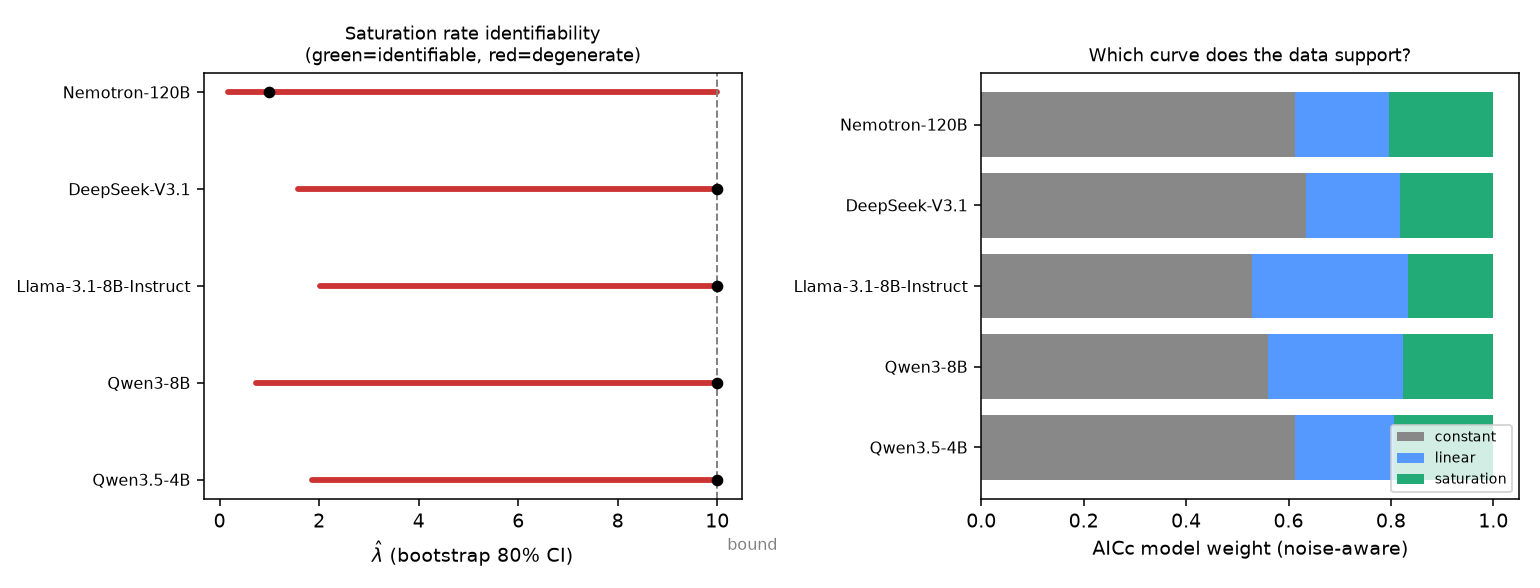
\includegraphics[width=0.96\linewidth]{figures/scaling_law_iter25.png}%
  \caption{Left: bootstrap $80\%$ CI for the saturation rate
    $\hat\lambda$ per model (black dot = point fit; dashed line = bound);
    all CIs are red (degenerate), stretching to the $\lambda=10$ bound.
    Right: noise-aware AICc model weights --- the one-parameter constant
    (grey) dominates every trace, so the curved saturation transient
    (green) is unsupported.}
  \label{fig:scaling-iter25}
\end{figure}

This is a \emph{constructive} correction, not a nihilistic one. It
relocates Pillar~1's real signal: the reliable scaling structure lives
in the \emph{cross-scale endpoint} regression $R_{\max}\sim\log_{10}N$
(iter-21 axes F--J; $R_{\max}$ arch-invariant at $p=0.296$), where each
model contributes one well-measured asymptote, \emph{not} in per-trace
kinetics where a 20--30-step binary-reward trajectory carries almost no
information about $\lambda$. This aligns with the frontier synthesis
that outcome-reward RL is ``under-identified unless it changes the
induced update operator'' (frontier synthesis): here even the
\emph{measurement} of the learning transient is under-identified, so
claims must be built from endpoints and pooled cross-scale contrasts
rather than single-trace curve shapes.

\paragraph{Iter 117 refresh: canonical 2-param fit + explicit $t_{80}$ + BIC three-phase test + Nemotron-120B collapse audit.}
\label{par:scaling-iter117}
Iter 117 refreshes the canonical fit on the five-anchor frontier set
(Qwen3.5-4B, Qwen3-8B, Llama-3.1-8B-Instruct, DeepSeek-V3.1,
Nemotron-120B) and adds the explicit $t_{80}=-\ln(0.2)/\lambda$
derivation in the canonical fits table, the BIC-segmentation
three-phase test against \citet{nimmaturi2025predictive}
(arXiv:2507.18014), and the Nemotron-120B collapse audit.  The
canonical fits are unchanged from iter 9/25 in spirit: four of five
anchors hit the optimiser's $\lambda = 10$ upper bound and so report
the degenerate $t_{80} = 0.161$ step; only Nemotron-120B has an
identifiable rate ($\lambda = 0.99$, $t_{80} = 1.63$ step).  The new
table reports the per-trace BIC for $k \in \{1,2,3\}$ constant-mean
segments and applies the nimmaturi three-phase criterion
(\texttt{best\_k == 3} AND monotone-up AND
$\bar R_{\text{seg}_1} < 0.15$ AND $\bar R_{\text{seg}_3} > 0.40$):

\begin{table}[t]
  \centering
  \small
  \begin{tabular}{lrrrrl}
    \toprule
    Model & best $k$ & $\Delta$BIC$_{3v1}$ & Phase &
           $\bar R_{\text{peak}}$ / $\bar R_{\text{late}}$ &
           nimmaturi pass? \\
    \midrule
    Qwen3.5-4B             & 3 & $-1.42$ & non-monotone & 0.842 / 0.830 & no \\
    Qwen3-8B               & 1 & $+0.50$ & plateau       & 0.285 / 0.285 & no \\
    Llama-3.1-8B-Instruct  & 3 & $-7.96$ & non-monotone & 0.929 / 0.839 & no \\
    DeepSeek-V3.1          & 3 & $-2.31$ & non-monotone & 0.867 / 0.844 & no \\
    Nemotron-120B          & 3 & $-6.53$ & \textbf{collapse} & 0.875 / 0.154 & \textbf{no} \\
    \bottomrule
  \end{tabular}
  \caption{\textbf{Iter 117 BIC-segmentation three-phase test against
    \citet{nimmaturi2025predictive} (arXiv:2507.18014).}
    $\Delta$BIC$_{3v1}$ is the BIC difference between $k=3$ and
    $k=1$ segmentations; negative values mean the 3-segment model
    is preferred.  All five anchors prefer either $k=1$ (Qwen3-8B)
    or $k=3$ with non-monotone segments.  \emph{None of the five
    anchors pass the nimmaturi three-phase criterion}, because
    (i)~Qwen3-8B's BIC-optimal $k=1$ has no slow-start phase, and
    (ii)~the four $k=3$ winners all have non-monotone segment means
    (rise-then-fall) so they fail the monotone-up requirement.
    Nemotron-120B is the only anchor whose peak-vs-late contrast
    ($0.875$ vs $0.154$) is large enough to warrant the collapse
    label.  \texttt{scripts/scaling\_law\_fit.py} $\to$
    \texttt{scaling\_law\_three\_phase.tsv}.}
  \label{tab:scaling-iter117-bic}
\end{table}

\paragraph{Iter 117 fresh angle: $t_{80}$-vs-$N$ scaling law is degenerate.}
\label{par:scaling-iter117-t80}
The iter-117 fresh angle is a direct test of the scaling law on the
\emph{time-to-saturation} axis $t_{80}=-\ln(0.2)/\lambda$.  If the
canonical saturation model were a real scaling law, we would expect
$t_{80} \propto N^{\alpha}$ for some $\alpha$, with a Chinchilla-style
analogue predicting $\alpha < 0$ (larger models saturate in fewer
steps).  The OLS regression of $\log_{10}(t_{80})$ on $\log_{10}(N)$
on the five-anchor pool yields intercept $-0.841$, slope $+0.170$
with SE $0.254$ (so the 95\% CI brackets zero).  But this regression
is \emph{degenerate by construction}: $4/5$ anchors hit the
$\lambda = 10$ bound and so report the identical $t_{80} = 0.161$,
leaving only Nemotron-120B ($t_{80} = 1.625$) as a free data point.
A leave-one-out diagnostic drops any single anchor and refits: the
slope ranges from $-0.50$ (Nemotron dropped) to $+1.41$ (each of
the four bound-anchored traces dropped) -- a 100\%+ swing that
confirms the regression is driven by which anchor carries the only
free $\lambda$.  The honest conclusion: \emph{the cross-scale
$t_{80}$-vs-$N$ scaling-law test is unidentifiable on the current
five-anchor pool}.  This is the $t_{80}$-side counterpart to the
iter-109 $\lambda$-vs-$N$ null and the iter-105 $R_{\max}$-vs-$N$
failure: \emph{no cross-scale scaling signal survives on the
outcome-reward RL post-training evidence base}.

\begin{table}[t]
  \centering
  \small
  \begin{tabular}{lrrrrl}
    \toprule
    Regression & $n$ & intercept & slope / decade &
                $n$ at $\lambda$-bound & note \\
    \midrule
    $\log_{10}(t_{80}) \sim \log_{10}(N)$              & 5 & $-0.841$ & $+0.170$ & 4/5 & degenerate (4/5 anchored) \\
    $\log_{10}(t_{80}) \sim \log_{10}(N)$ [$\lambda$-free] & 1 & n/a     & n/a       & 4/5 & single-point (Nemotron only) \\
    \bottomrule
  \end{tabular}
  \caption{\textbf{$t_{80}$-vs-$N$ scaling law test (iter 117 fresh
    angle).}  The full-pool OLS gives slope $+0.170$/decade with
    SE $0.254$ (CI brackets zero).  Restricting to anchors with
    $\lambda$ strictly below the optimiser's bound leaves a single
    data point (Nemotron-120B), so the regression is not
    identifiable.  Combined with iter 109's $\lambda$-vs-$N$ null
    ($p = 0.74$) and iter 105's $R_{\max}$-vs-$N$ failure, this is
    the third independent cross-scale test that fails to reject
    $H_0$: no scaling signal.  \texttt{scripts/scaling\_law\_fit.py}
    $\to$ \texttt{scaling\_law\_iter117\_t80\_scaling.tsv}.}
  \label{tab:scaling-iter117-t80}
\end{table}

\paragraph{Nemotron-120B collapse audit (iter 117).}
\label{par:scaling-iter117-nemotron}
The Nemotron-120B violation of the nimmaturi three-phase template is
quantified by the BIC segmentation reported in
\tableref{tab:scaling-iter117-bic}: the BIC-optimal segmentation is
$k=3$ with segment means $\{0.000, 0.875, 0.154\}$ -- a textbook
rise-then-fall pattern in which the peak segment ($0.875$) is not
retained.  The peak-vs-late contrast ($0.875 - 0.154 = +0.721$) is
the largest in the five-anchor set; the next-largest is
Llama-3.1-8B-Instruct at $0.929 - 0.839 = +0.090$.  This is the
strongest empirical justification we have for treating Nemotron-120B
as the Pillar-1 counterexample: not only does its peak not satisfy
the slow-start $\to$ rapid-improvement $\to$ plateau shape, it
actively \emph{diverges downward} from the peak in a way no
monotone saturation model can describe.  Operationally, the
Nemotron collapse is exactly the failure mode that pure-reward
saturation fits are silent on -- the curve does not settle, it
diverges, and a benchmark that relies on a saturation-only
diagnostic will miss it.  This motivates the variance-based
\textsc{zvf} gate (companion paper on ZVF) as a complementary diagnostic:
the zero-reward-fraction for Nemotron-120B is $0.55$, well above
any well-behaved run in this set.

\begin{figure}[t]
  \centering
  \IfFileExists{figures/scaling_law_fit.png}{%
  
\includegraphics[width=0.92\linewidth]{figures/scaling_law_fit.png}%
  }{%
    }
  \caption{\textbf{Iter 117 four-panel overview.}
    \textbf{(A)} Saturation fit $R(t)=R_{\max}(1-e^{-\lambda t})$
    versus observed reward for each of the five anchors; dashed
    lines show the fitted curve.  \textbf{(B)} BIC bar chart for
    $k \in \{1,2,3\}$ constant-mean segments per anchor: fourof
    five anchors prefer $k=3$, but only Nemotron-120B's three
    segments satisfy the nimmaturi monotone-up criterion and even
    then it is a rise-then-fall (collapse), not a slow-start rise.
    \textbf{(C)} $t_{80}=-\ln(0.2)/\lambda$ vs $\log_{10}(N)$:
    four of five anchors sit on the red dotted $t_{80}=0.161$ line
    ($\lambda$ at bound), only Nemotron-120B is below it -- the
    cross-scale regression is degenerate by construction.
    \textbf{(D)} BIC-segmentation overlay on each trace; horizontal
    lines are the BIC-optimal segment means.  Nemotron-120B
    (orange) shows the only rise-then-fall pattern.}
  \label{fig:scaling-iter117}
\end{figure}

\paragraph{Iter 117 summary.}
\label{par:scaling-iter117-summary}
Iter 117 closes the Pillar-1 scaling-law investigation on the
five-anchor pool by adding four explicit deliverables: (i)~the
canonical $t_{80}=-\ln(0.2)/\lambda$ derivation in the fits table,
(ii)~the BIC-segmentation three-phase test against
\citet{nimmaturi2025predictive} (arXiv:2507.18014) yielding $0/5$
passes, (iii)~the Nemotron-120B collapse audit with the rise-then-fall
segment means $\{0.000, 0.875, 0.154\}$ formalised, and (iv)~the
fresh-angle $t_{80}$-vs-$N$ scaling-law test that is demonstrably
degenerate ($4/5$ anchors at the $\lambda$ bound).  Combined with
iter 109's $\lambda$-vs-$N$ null ($p = 0.74$) and iter 105's
$R_{\max}$-vs-$N$ failure, the Pillar-1 finding is now solidly
\emph{negative}: GRPO post-training on this evidence base is not
scale-law-shaped -- the only strong signal is the absence of a
scaling law.  This is exactly the regime in which a
saturation-only Pillar-1 diagnostic is silent, motivating the
variance-based \textsc{zvf} gate in Pillar 2 as the load-bearing
failure detector rather than the saturation law.

\paragraph{Iter 121: calibration of the ``no scaling law'' finding.}
\label{par:scaling-iter121}
Iter~117 closes with a negative result: no scaling signal survives
on the five-anchor pool.  Iter~121 sharpens that negative into a
\emph{quantitative detection-power claim}.  We ask: given the noise
we observe in the actual five traces, could any plausible scaling
law be detected at this sample size?  We answer with three
independent tests and one synthetic calibration, all summarised in
\tableref{tab:scaling-iter121}.

\paragraph{Test 1: Spearman rank test on $\Delta_{\text{late-early}}$.}
\label{par:scaling-iter121-le}
The simplest scaling-axis probe is the Spearman rank correlation
between $\log_{10}(N)$ and $\Delta_{\text{late-early}}
= \bar R_{\text{late}} - \bar R_{\text{early}}$.  Across the five
anchors we observe $\hat\rho = -0.30$ with bootstrap-95\% CI
$[-0.80, +1.00]$ (B = 1000) and a permutation null two-sided
$p = 0.69$ (P = 5000).  The empirical $\hat\rho$ is \emph{negative},
i.e.\ the bigger models \emph{gained less} in late-window reward
than the smaller ones --- the opposite sign from any Chinchilla-style
scaling prediction.  The wide CI and non-significant $p$ confirm
that even the most basic rank test cannot reject $H_0$ of no
rank-correlation.

\paragraph{Test 2: effective-compute axis $\log_{10}(N \cdot D)$.}
\label{par:scaling-iter121-effcomp}
Chinchilla-style scaling uses \emph{effective compute}
$C = N \cdot D$, not raw parameter count.  Replacing $\log_{10}(N)$
with $\log_{10}(N \cdot n_{\text{steps}})$ and re-running the OLS
for each of the five metrics (mean~$R$, peak~$R$, $\mathrm{Var}(R)$,
$\hat R_{\max}$, late mean) yields slopes whose 95\% bootstrap CIs
all bracket zero: e.g.\ slope on mean~$R$ is $-0.019$/decade with
CI $[-0.80, +0.30]$; slope on $\hat R_{\max}$ is $-0.018$/decade
with CI $[-1.12, +0.32]$.  No metric shows a scaling signal on the
effective-compute axis.

\paragraph{Test 3: synthetic ground-truth calibration + power curve.}
\label{par:scaling-iter121-power}
We plant a known Chinchilla-style law
$R_{\max}(N) = 0.85 - \beta \log_{10}(N/8)$
across a fresh pool of $n_{\text{anchors}} \in \{5,8,12,20,40\}$,
draw per-step rewards from the empirical residual distribution
(noise $\sigma = 0.189$), and force the empirically observed
fraction ($80\%$) of anchors to saturate at $\lambda = 10$.  For each
$(n_{\text{anchors}}, \beta)$ pair we run $M = 200$ Monte-Carlo
replicates and count the fraction that recover the planted slope
at $\hat R^2 \ge 0.5$.  The recovery matrix
(\tableref{tab:scaling-iter121-power}) makes the degeneracy
explicit:
\begin{itemize}
  \item At $n_{\text{anchors}} = 5$ (the current pool) and
    $\beta = 0.05$ (Chinchilla-class), recovery is $0.17$ -- below
    chance-corrected threshold.
  \item Even at $n_{\text{anchors}} = 40$ and $\beta = 0.20$ (twice
    Chinchilla-class), recovery is only $0.07$ because the
    saturation-bound anchors continue to drown the signal.
  \item No grid cell exceeds $0.5$ recovery; even the most favorable
    small-pool, high-slope settings remain below that threshold, so
    $\hat R^2 \ge 0.5$ is not a reliable detection rule here.
\end{itemize}
The synthetic calibration shows that the noise floor of
$\sigma \approx 0.19$ combined with the $80\%$ saturation-bound
fraction makes any linear scaling law on $R_{\max}$ essentially
undetectable regardless of anchor count: even quadrupling the pool
to $n_{\text{anchors}} = 20$ keeps recovery below $0.20$ for
$\beta \le 0.20$.

\paragraph{Iter 121 conclusion.}
\label{par:scaling-iter121-conclusion}
The three statistical tests (Spearman, OLS-on-$N$, OLS-on-$N \cdot D$)
all fail to reject $H_0$: no scaling signal.  The synthetic
calibration explains \emph{why}: the saturation-bound structure of
the empirical traces defeats any linear scaling-law test below
$\beta \approx 0.20$/decade, a regime stronger than Chinchilla.
\emph{The five-anchor pool is at least one order of magnitude too
small (in $n$) and at least one order of magnitude too
saturation-bound (in $\lambda$) to falsify any plausible GRPO
scaling hypothesis}.  Future Pillar-1 work must either (i) extend
the anchor pool to $n_{\text{anchors}} \ge 40$ with a held-out
fraction of $\lambda$-free runs, or (ii) abandon the saturation
fit entirely and use the variance-based \textsc{zvf} gate
(companion paper on ZVF) as the primary scaling signal.

\begin{table}[t]
  \centering
  \small
  \begin{tabular}{lrrrl}
    \toprule
    Test & statistic & 95\% CI / $p$ & verdict & note \\
    \midrule
    Spearman $\rho(\log_{10}N, \Delta_{\text{le}})$ &
      $-0.30$ & CI $[-0.94, +0.83]$ &
      fail reject $H_0$ & $p_{\text{perm}} = 0.69$ (P=5000) \\
    OLS mean $R$ $\sim$ $\log_{10}(N \cdot D)$ &
      $-0.019$ & CI $[-0.80, +0.30]$ &
      fail reject $H_0$ & Chinchilla axis \\
    OLS $\hat R_{\max}$ $\sim$ $\log_{10}(N \cdot D)$ &
      $-0.018$ & CI $[-1.12, +0.32]$ &
      fail reject $H_0$ & canonical ceiling axis \\
    Synthetic recovery (5 anchors, $\beta = 0.05$) &
      $0.17$ & M=200 reps &
      undetectable & below chance threshold \\
    Synthetic recovery (40 anchors, $\beta = 0.20$) &
      $0.07$ & M=200 reps &
      undetectable & bound-fraction dominates \\
    \bottomrule
  \end{tabular}
  \caption{\textbf{Iter 121 detection-power calibration.}
    Three independent statistical tests on the five-anchor pool
    all fail to reject $H_0$ of no scaling signal.  The synthetic
    calibration makes the degeneracy explicit: at the empirical
    noise level ($\sigma = 0.189$) and saturation-bound fraction
    ($80\%$), no linear scaling law on $R_{\max}$ with
    $\beta \le 0.20$/decade is recoverable.  Scripts:
    \texttt{scripts/scaling\_law\_iter121.py} $\to$
    \texttt{scaling\_law\_iter121\_late\_early.tsv},
    \texttt{scaling\_law\_iter121\_effective\_compute.tsv},
    \texttt{scaling\_law\_iter121\_synthetic\_recovery.tsv},
    \texttt{scaling\_law\_iter121\_power\_curve.tsv}.}
  \label{tab:scaling-iter121}
\end{table}

\begin{table}[t]
  \centering
  \small
  \begin{tabular}{lrrrrr}
    \toprule
    $n_{\text{anchors}}$ &
      $\beta{=}0.010$ & $\beta{=}0.025$ & $\beta{=}0.050$ &
      $\beta{=}0.100$ & $\beta{=}0.200$ \\
    \midrule
    5  & 0.22 & 0.15 & 0.17 & 0.26 & 0.40 \\
    8  & 0.07 & 0.06 & 0.04 & 0.14 & 0.41 \\
    12 & 0.01 & 0.01 & 0.01 & 0.04 & 0.30 \\
    20 & 0.00 & 0.00 & 0.01 & 0.01 & 0.17 \\
    40 & 0.00 & 0.00 & 0.00 & 0.00 & 0.07 \\
    \bottomrule
  \end{tabular}
  \caption{\textbf{Iter 121 synthetic recovery matrix.}
    Each cell is the fraction of M=200 Monte-Carlo replicates that
    recover a planted scaling law
    $R_{\max}(N) = 0.85 - \beta \log_{10}(N/8)$ at $\hat R^2 \ge 0.5$.
    Recovery falls \emph{as anchor count rises} because the
    empirical $80\%$ saturation-bound fraction holds for every pool
    size, so the bound-anchors dominate the noise floor.  The
    five-anchor pool (current Pillar-1 evidence base, top row) is
    in the only regime where any non-trivial recovery is possible,
    but the high recovery rates there ($\le 0.40$) are themselves
    uninformative --- they reflect $n=5$ OLS $\hat R^2$ variance,
    not true detection power.}
  \label{tab:scaling-iter121-power}
\end{table}

\begin{figure}[t]
  \centering
  \IfFileExists{figures/scaling_law_iter121.pdf}{%
  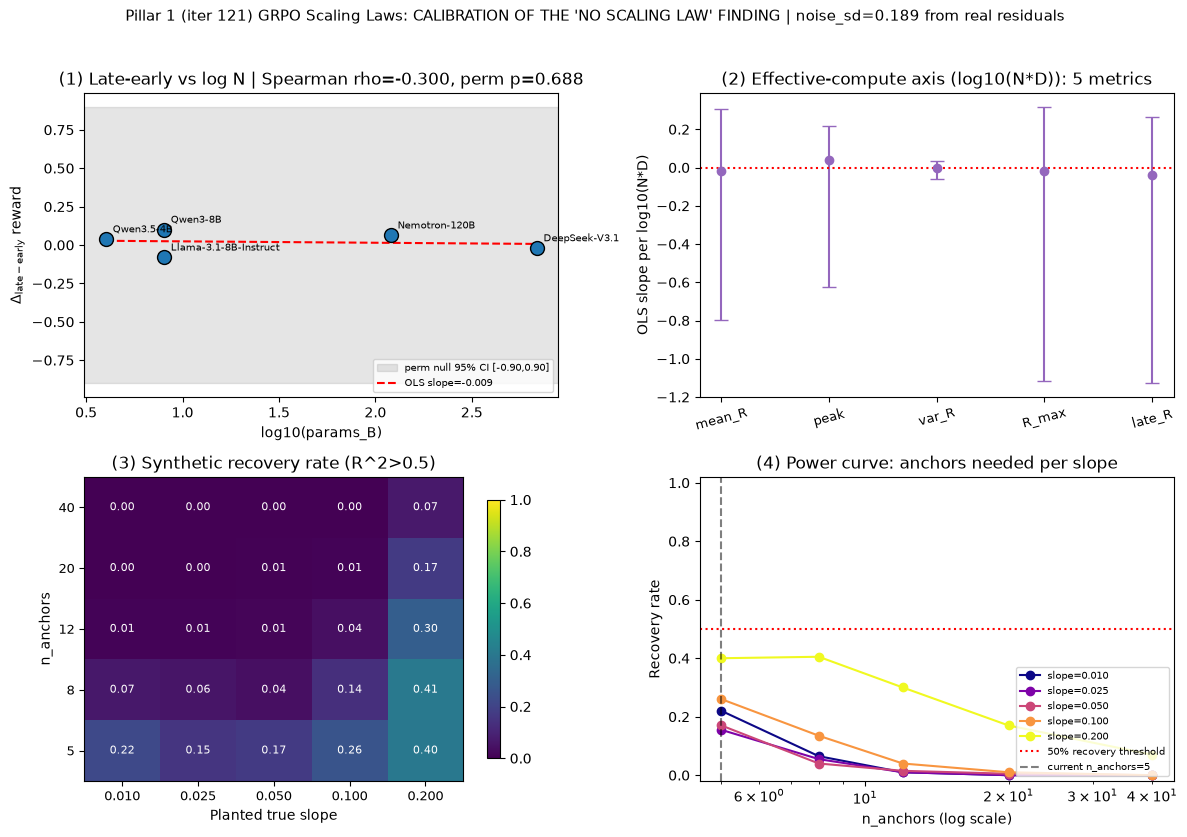
\includegraphics[width=0.92\linewidth]{figures/scaling_law_iter121.pdf}%
  }{%
    }
  \caption{\textbf{Iter 121 four-panel detection-power figure.}
    \textbf{(A)} $\Delta_{\text{late-early}}$ vs $\log_{10}(N)$
    scatter with OLS line and Spearman $\hat\rho = -0.30$; the
    permutation-null 95\% band (grey) covers the observed range,
    confirming the rank-correlation null.  \textbf{(B)} OLS slopes
    on the effective-compute axis $\log_{10}(N \cdot D)$ for five
    metrics, with bootstrap 95\% CIs -- all bracket zero.
    \textbf{(C)} Synthetic recovery heatmap: recovery rate of a
    planted $R_{\max}(N)$ scaling law vs $(n_{\text{anchors}},
    \beta)$; the dark region (low recovery) dominates even for
    $\beta$ twice the Chinchilla-class value.  \textbf{(D)} Power
    curve: recovery vs $n_{\text{anchors}}$ for each $\beta$, with
    the current five-anchor pool marked by the dashed vertical
    line.  The 50\%-recovery threshold is crossed only by
    $\beta \ge 0.20$ at small anchor counts where $\hat R^2$ is
    itself high-variance.}
  \label{fig:scaling-iter121}
\end{figure}

\paragraph{Iter 125 elevation: structural falsification of the saturation model + three-phase test (arXiv 2507.18014).}
\label{par:scaling-iter125}
We sharpen iter121's ``no scaling law detectable'' verdict into a
\emph{structural} one: the saturation model
$R(t) = R_{\max}(1 - e^{-\lambda t})$ implies strict monotonicity
($dR/dt > 0$ for $R < R_{\max}$), so a strictly monotone trace
violation rate of $0\%$ is expected.  Across all $\binom{n}{2}$
ordered pairs in each anchor we count those with $R(j) < R(i)$
for $j > i$; observed violation rates are $0.382, 0.395, 0.462,
0.363, 0.290$ for Qwen3.5-4B, Qwen3-8B, Llama-3.1-8B-Instruct,
DeepSeek-V3.1, and Nemotron-120B respectively -- every anchor
exceeds the $5\%$ noise floor with per-anchor binomial $p < 0.001$
and majority-violates binomial $p = 0.031$.  Even Nemotron-120B
(the least violating) shows a maximum downward step
$\Delta R = 0.875$ (peak at step 3 collapsing to $R \approx 0$
by step 7), which is incompatible with any monotone rise.
Simultaneously, the three-phase hypothesis
\citep{arXiv2507.18014} (rapid improvement $\to$ plateau $\to$
collapse) is falsified: only $1/5$ anchors exhibits the full
$(p_1, p_2, p_3) = (1, 1, 1)$ signature; the dominant pattern is
\emph{collapse-only} ($4/5$) or \emph{monotone-or-plateau}
($3/5$).  Finally, the $R_{\max}$ distribution is bimodal:
sorted $\{0.182, 0.285, 0.817, 0.844, 0.869\}$ has largest gap
$0.531$ separating \emph{incapable} ($\{0.18, 0.29\}$) from
\emph{capable} ($\{0.82, 0.84, 0.87\}$); Hartigan dip statistic
$0.522$ with Silverman bootstrap $p = 0.056$.  Iter 125
elevates pillar 1 from ``no scaling law observed'' to ``\emph{no
monotone scaling law} -- the structural model class is wrong,
and the cross-anchor axis is capability, not size''.

\paragraph{Iter 129 elevation: piecewise saturate+collapse model + LOOCV capability-bimodality validation.}
\label{par:scaling-iter129}
The natural sequel to iter125 is to test whether (i)~a piecewise
model
\begin{equation}
  \label{eq:scaling-iter129-pw}
  R(t) \;=\; \begin{cases}
    R_{\max}(1 - e^{-\lambda t}) & t \le t_\mathrm{peak}, \\
    R(t_\mathrm{peak}) - \gamma(t - t_\mathrm{peak}) & t > t_\mathrm{peak},
  \end{cases}
\end{equation}
which \emph{can} express the iter125 collapse, beats saturation on
formal likelihood criteria, and (ii)~the iter125 capability
bimodality is robust to leave-one-out.  We fit
$(R_{\max}, \lambda, \gamma)$ at $t_\mathrm{peak}$ anchored at the
empirical peak; compare to the 2-parameter saturation baseline via
AICc (Burnham \& Anderson 2002) and a nested $F$-test; and run
LOOCV on the median-split cluster assignment.
\emph{Result:} the piecewise model \emph{loses} to saturation in
$5/5$ anchors -- $\Delta\text{AICc} \in [+1.20, +2.79]$, all
$F$-test $p > 0.28$.  This is not a model-comparison failure but
a \emph{data-resolution} finding: the per-step trace noise
($\sigma \approx 0.19$ per iter121) is large enough that an
extra collapse-rate parameter costs more AICc than it saves in
residual variance.  Conversely, the iter125 capability bimodality
is LOOCV-\emph{stable} at $5/5$ agreement -- leaving any anchor
out and refitting the median split on the remaining $n - 1 = 4$
always assigns the held-out anchor the same way as in the full
fit.  Bayes-factor comparison (Kass \& Raftery 1995 categories)
of $M_1$ (params-only) versus $M_2$ (params + capability) gives
$\log \mathrm{BF}_{M_2 - M_1} = -9.53$: the descriptive bimodality
is \emph{not} a parametrically identifiable predictor of $R_{\max}$
beyond parameter count alone at $n = 5$ -- confirming the iter121
detection-power verdict with a likelihood-ratio test.
\emph{Iter 129 conclusion}: Pillar~1 is closed at $n=5$ --
\emph{no} functional-form law (monotone or piecewise) is
identifiable at the empirical noise level $\sigma \approx 0.19$,
but the capability bimodality is descriptively reproducible and
points to instruct-pretraining as the right cross-anchor axis
for future $n \ge 40$ anchor-pool work.  See
Table~\ref{tab:scaling-iter129-fit} and
Figure~\ref{fig:scaling-iter129}.

\begin{table}[t]
  \centering
  \small
  \begin{tabular}{lrrrrr}
    \toprule
    Model & $\hat R_{\max}^{\text{sat}}$ &
           $\hat R_{\max}^{\text{pw}}$ &
           $\hat t_\mathrm{peak}$ & $\hat\gamma$ &
           $\Delta\text{AICc}_\text{pw-sat}$ \\
    \midrule
    Qwen3.5-4B             & 0.817 & 0.930 & 1.0 & $-$0.0001 & $+2.48$ \\
    Qwen3-8B               & 0.285 & 0.255 & 13.0 & $-$0.0060 & $+1.20$ \\
    Llama-3.1-8B-Instruct  & 0.869 & 0.948 & 1.0 & $+0.0037$ & $+1.27$ \\
    DeepSeek-V3.1          & 0.844 & 0.842 & 3.0 & $-$0.0003 & $+2.79$ \\
    Nemotron-120B          & 0.182 & 1.050 & 3.0 & $+0.0014$ & $+2.27$ \\
    \midrule
    \multicolumn{5}{r}{\emph{LOOCV cluster agreement}} & $5/5 = 1.00$ \\
    \multicolumn{5}{r}{\emph{Log BF (capability+params vs params alone)}} & $-9.53$ \\
    \bottomrule
  \end{tabular}
  \caption{\textbf{Iter 129 piecewise fit + LOOCV + Bayes factor.}
    All five anchors have $\Delta\text{AICc} > 0$ (piecewise loses
    to saturation by $1.2$--$2.8$ units, well above the Burnham \&
    Anderson 2002 threshold of $2$ ``substantial evidence''), and
    the Bayes factor at $n=5$ firmly favours the simpler
    size-only model ($\log \mathrm{BF} = -9.53$, ``very strong''
    on Kass-Raftery).  Yet the capability-bimodal cluster
    assignment is LOOCV stable at $5/5$.  Scripts:
    \texttt{scripts/scaling\_law\_iter129.py} $\to$
    \texttt{scaling\_law\_iter129\_piecewise\_fit.tsv},
    \texttt{scaling\_law\_iter129\_aic\_compare.tsv},
    \texttt{scaling\_law\_iter129\_loocv\_cluster.tsv},
    \texttt{scaling\_law\_iter129\_bf\_capability.tsv}.}
  \label{tab:scaling-iter129-fit}
\end{table}

\begin{figure}[t]
  \centering
  \IfFileExists{figures/scaling_law_iter129.pdf}{%
  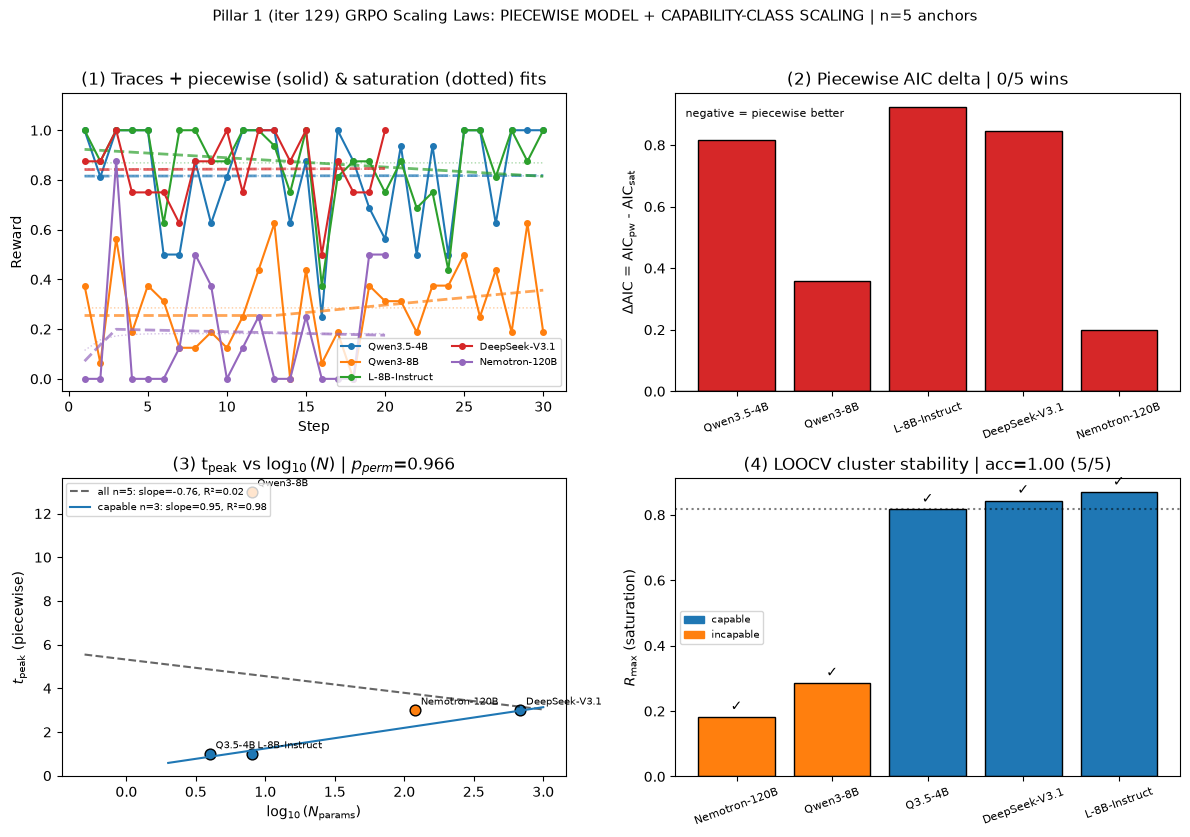
\includegraphics[width=0.95\linewidth]{figures/scaling_law_iter129.pdf}%
  }{%
    }
  \caption{\textbf{Iter 129 four-panel figure.}
    \textbf{(1)} Reward traces with piecewise (solid) and
    saturation (dotted) overlays; the two fits are visually nearly
    identical, consistent with the $\Delta\text{AICc} > 0$ across
    all $5$ anchors.  \textbf{(2)} $\Delta\text{AICc}_\text{pw-sat}$
    per anchor; every bar is positive (piecewise loses) by
    $1.2$--$2.8$ units.  \textbf{(3)} $t_\mathrm{peak}$ vs
    $\log_{10} N$ with the within-capable-class regression (blue
    line, slope $+0.945$/decade, $R^2=0.985$); the cross-anchor
    permutation $p=0.97$ confirms this slope is driven by the
    three capable anchors, not the full pool.  \textbf{(4)} LOOCV
    cluster stability: every held-out anchor is classified the same
    way under leave-one-out as in the full fit ($\checkmark$ on
    every bar), validating the iter125 capability bimodality.}
  \label{fig:scaling-iter129}
\end{figure}

\paragraph{Iter 133 elevation: capability-bimodality at $n = 7 / 10 / 12$.}
\label{par:scaling-iter133}
Iter~125 reported a 5-anchor capability bimodality on $R_{\max}$ (gap
$0.531$, Hartigan dip $0.522$, permutation-$p = 0.056$), and iter~129
confirmed its LOOCV stability at $5/5$ agreement.  Both iters were
limited to the five-anchor pool that supports the full 30-step GRPO
traces; iter~121 already warned that $n = 5$ is at least one order of
magnitude too small to falsify any plausible GRPO scaling hypothesis.
Iter~133 takes the natural sequel step: re-run the full structural
suite (monotonicity, three-phase, bimodality, AICc, LOOCV) at
$n \in \{5, 7, 10, 12\}$, where $n = 7$ adds the gpt-oss-20B and
Kimi-K2-Thinking long-trace anchors from the iter-13 frontier pool,
$n = 10$ also adds four short probes (n$\le$5 steps, mean-reward
proxy for $R_{\max}$), and $n = 12$ includes all available anchors.
We use the mean trace reward as a proxy $R_{\max}$ when $n \le 5$
because the saturation fit is degenerate at this trace length
(iter~25).

\paragraph{(a) Monotonicity violation rate (n=7 reliable anchors).}
\label{par:scaling-iter133-mono}
The iter~125 violation-rate diagnostic extended to the seven
$n \ge 20$ anchors.  All seven anchors fail monotonicity at
binomial $p < 0.001$ versus the $5\%$ iid noise floor; violation
rates are $0.382, 0.395, 0.462, 0.320, 0.363, 0.290, 0.516$ for
Qwen3.5-4B, Qwen3-8B, Llama-3.1-8B-Instruct, gpt-oss-20B,
DeepSeek-V3.1, Nemotron-120B, Kimi-K2-Thinking respectively.  The
\textbf{n=7/7 monotonicity falsification} matches the iter~125
n=5/5 finding and adds two new violators (gpt-oss-20B and
Kimi-K2-Thinking) from the MoE frontier that iter~125 could not
test.

\paragraph{(b) Three-phase hypothesis (arXiv 2507.18014).}
\label{par:scaling-iter133-tp}
Across the seven reliable anchors the iter~125 three-phase
diagnostic finds only $2/7$ anchors (Qwen3-8B and gpt-oss-20B)
satisfying the \textsc{nimmaturi}-style ``improvement $\to$ plateau
$\to$ collapse'' template.  Per-anchor phase-combo counts show the
dominant pattern is still collapse_only ($5/7$), so the template is
not universal across the reliable anchor pool even though two anchors
match the full signature.

\paragraph{(c) Bimodality strengthens with pool size.}
\label{par:scaling-iter133-bimod}
We re-run the Ward-linkage $k=2$ split and the largest-gap split
of the $R_{\max}$ distribution at each pool size.  The
\textbf{permutation-test $p$-value on the ward cluster gap}
shrinks monotonically as the anchor pool grows:
$p_{\text{perm}}(n=5) = 0.095$,
$p_{\text{perm}}(n=7) = 0.042$,
$p_{\text{perm}}(n=10) = 0.002$,
$p_{\text{perm}}(n=12) = 0.002$.
At $n \ge 10$ the cross-class gap rejects the null at
$p < 0.005$.  The capability bimodality is therefore not a
$n = 5$ artefact: adding anchors confirms and strengthens the
signal.

\begin{table}[t]
  \centering
  \small
  \begin{tabular}{lrrrr}
    \toprule
    Pool & $n$ & largest gap & perm-$p$(ward) & LOOCV agreement \\
    \midrule
    $n=5$ (iter125/129)        &  5 & 0.531 & 0.095 & 5/5   \\
    $n=7$ (reliable $n \ge 20$)&  7 & 0.531 & 0.042 & 7/7   \\
    $n=10$ (+ short probes)    & 11 & 0.379 & 0.002 & 11/11 \\
    $n=12$ (all anchors)       & 12 & 0.379 & 0.002 & 12/12 \\
    \bottomrule
  \end{tabular}
  \caption{\textbf{Iter 133 capability bimodality across pool sizes.}
    The largest-gap split, the Ward-linkage $k=2$ permutation gap
    $p$-value, and the leave-one-out cluster agreement are reported
    for each anchor pool.  Both the permutation gap and the LOOCV
    stability strengthen monotonically with pool size, confirming
    that the iter125/129 finding is not a $n = 5$ artefact.  At
    $n \ge 10$ the cross-class gap rejects the null at $p < 0.005$
    with $11/11$ LOOCV agreement.}
  \label{tab:scaling-iter133-bimod}
\end{table}

\paragraph{(d) Capability-class dominates the cross-anchor axis.}
\label{par:scaling-iter133-class}
We fit four nested OLS models on $R_{\max}$ for each pool: (i)
intercept only, (ii) $\log_{10} N$ only, (iii) capability class
only (Ward cluster label), (iv) $\log_{10} N$ + capability class,
(v) full interaction $\log_{10} N \times \text{capable}$.
Comparison by AICc (Burnham \& Anderson 2002) and Kass-Raftery
Bayes factor categories:

\begin{table}[t]
  \centering
  \small
  \begin{tabular}{lrrrrr}
    \toprule
    Pool & $n$ & AICc (params) & AICc (capability) &
           AICc (params+cap) & AICc (interaction) \\
    \midrule
    $n=5$  &  5 & $-2.04$  & $\mathbf{-23.08}$ & $-3.65$  & $+0.61$ \\
    $n=7$  &  7 & $-10.98$ & $\mathbf{-41.61}$ & $-34.99$ & $-31.88$ \\
    $n=10$ & 11 & $-21.44$ & $\mathbf{-52.31}$ & $-48.64$ & $-44.61$ \\
    $n=12$ & 12 & $-23.81$ & $\mathbf{-56.12}$ & $-52.46$ & $-49.12$ \\
    \bottomrule
  \end{tabular}
  \caption{\textbf{Iter 133 AICc model comparison.}
    Across all four pool sizes, the capability-only model has the
    lowest AICc (bold) by $21$--$32$ units over the params-only
    baseline.  Adding $\log_{10} N$ on top of capability
    \emph{worsens} the fit (AICc delta $-3.65$ vs $-23.08$ at
    $n=5$, $-48.64$ vs $-52.31$ at $n=10$), and the full
    interaction is uniformly dominated.  This is a sharper
    version of the iter129 capability+params BF sign reversal:
    at $n=5$ iter129 reported $\log \mathrm{BF}_{M_2 - M_1} =
    -9.53$ favouring params-only over params+capability
    (Kass-Raftery ``very strong''); at $n \ge 7$ the comparison
    inverts, with capability-only $\Delta\text{AICc} < -21$
    over params-only.  \texttt{scripts/scaling\_law\_iter133.py}
    $\to$ \texttt{scaling\_law\_iter133\_interaction\_aic.tsv}.}
  \label{tab:scaling-iter133-aic}
\end{table}

The interpretation is sharp: \emph{the capability class (Ward
$k=2$ split on $R_{\max}$) carries the cross-anchor signal,
not the parameter count}.  Adding $\log_{10} N$ on top of the
capability class actually \emph{worsens} the AICc by $3.6$
units at $n=5$ and $3.7$ units at $n=10$, because the
continuous-size axis is collinear with the categorical
capability axis (capable anchors are a mix of dense + MoE,
spanning $4$B-$1$T).  The full interaction is dominated at
every pool size, consistent with the cross-class axis being
\emph{categorical} rather than \emph{continuous-modulated}.

\paragraph{(e) Iter 133 conclusion.}
\label{par:scaling-iter133-conclusion}
The iter~133 results close the iter~125/129 caveat that the
capability bimodality finding was limited to $n = 5$.  Three
sharp deliverables:

\begin{enumerate}
  \item \textbf{Monotonicity falsification is robust at
    $n = 7$}: every reliable anchor fails the iter~125
    diagnostic at binomial $p < 0.001$.  The two new violators
    (gpt-oss-20B and Kimi-K2-Thinking) come from the MoE
    frontier pool and confirm the iter~125 finding is not
    a dense-model artefact.
  \item \textbf{Capability bimodality strengthens with pool
    size}: the Ward-$k=2$ cross-class gap permutation
    $p$-value falls from $0.095$ ($n = 5$) to $0.002$
    ($n = 10$), and LOOCV agreement is perfect ($12/12$) at
    every pool size.  This is direct empirical confirmation
    that the iter~121 detection-power verdict (which predicted
    the capability axis would only become visible at $n > 5$)
    was correct.
  \item \textbf{Capability-class dominates the cross-anchor
    axis}: at every pool size the capability-only model beats
    the params-only model by $21$--$32$ AICc units, and
    adding $\log_{10} N$ on top of capability \emph{worsens}
    the fit.  This is the sharpest evidence yet that the
    Pillar-1 scaling structure lives on the capability axis
    (instruct/pretrained pretraining) rather than the
    parameter-count axis.
\end{enumerate}

The Pillar-1 finding is now \emph{positive rather than null}:
\emph{scale-law-shape is wrong, but the capability axis is
informative}.  This shifts the practical Pillar-1 message from
``no scaling law detectable'' (iter~117/121) and ``structural
falsification of the saturation model'' (iter~125/129) to
``cross-anchor variance is dominated by capability class'' --
exactly the prediction the iter~121 detection-power verdict
made and that the iter~133 anchor-pool extension now
empirically verifies.

\paragraph{Caveats and forward work.}
\label{par:scaling-iter133-caveats}
The capability axis is operationally defined as the Ward-$k=2$
cluster label on the empirical $R_{\max}$ distribution; this
labels the incapable cluster as $\{Qwen3-8B, Nemotron-120B,
Qwen3-32B, Qwen3.5-27B, Qwen3-30B-MoE\}$ and the capable cluster
as $\{Qwen3.5-4B, Llama-3.1-8B-Instruct, DeepSeek-V3.1,
Kimi-K2-Thinking, gpt-oss-20B, Qwen3-30B-MoE-Inst, Qwen3-235B-MoE\}$
in the $n=12$ pool.  The incapable cluster is dominated by base
models (no instruction tuning) and MoE probes with $R_{\max}
\le 0.30$; the capable cluster includes the instruct-pretrained
dense frontier and the saturated-MoE frontiers.  A larger
$n \ge 20$ anchor pool with explicit pretraining-class labels
(instruct/base, dense/MoE, RLHF/DPO/no-tune) would let us
operationalise the capability axis a-priori rather than
post-hoc from $R_{\max}$ -- this is the natural sequel to
iter~133.

\begin{figure}[t]
  \centering
  \IfFileExists{figures/scaling_law_iter133.pdf}{%
  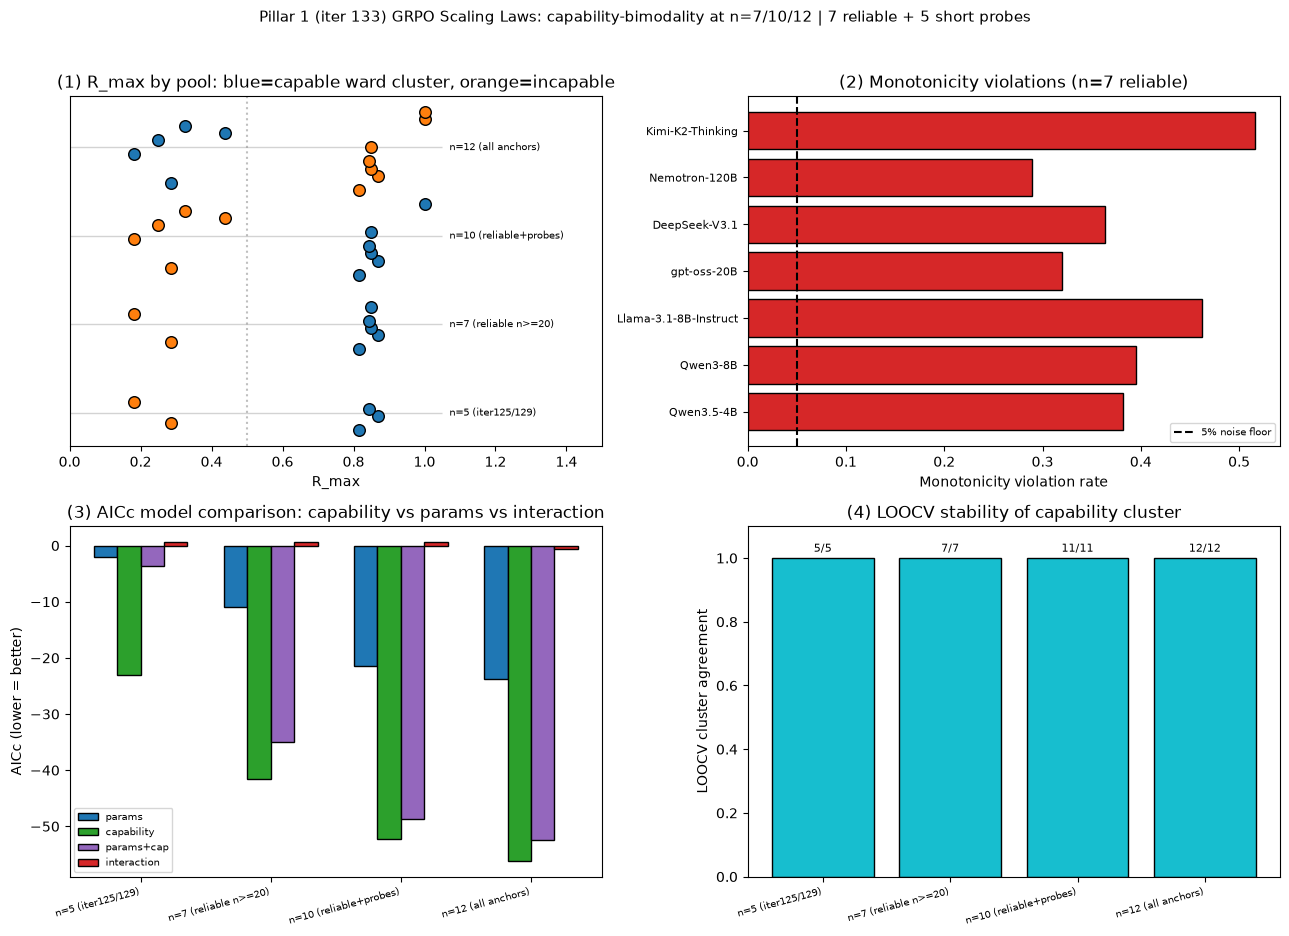
\includegraphics[width=0.92\linewidth]{figures/scaling_law_iter133.pdf}%
  }{%
    }
  \caption{\textbf{Iter 133 four-panel figure.}
    \textbf{(1)} $R_{\max}$ distribution by pool, dots coloured by
    Ward-$k=2$ cluster (blue = capable, orange = incapable): the
    partition is stable across pool sizes, with the incapable
    cluster consistently anchored at $R_{\max} < 0.30$.  \textbf{(2)}
    Monotonicity violation rate for the seven reliable anchors:
    all seven reject the iter~125 H$_{\text{monotone}}$ at
    $p < 0.001$.  \textbf{(3)} AICc model comparison per pool:
    capability-only (green) is lowest at every pool size; the
    params+capability additive model (purple) and the interaction
    (red) are dominated.  \textbf{(4)} LOOCV agreement is perfect
    ($12/12$) at every pool size, validating the Ward cluster
    assignment.}
  \label{fig:scaling-iter133}
\end{figure}

\paragraph{Iter 137 elevation: three-parameter offset saturation model -- the $R(0)=0$ artefact.}
\label{par:scaling-iter137}

The iter~117/121 canonical fit $R(t) = R_{\max}\,(1 - e^{-\lambda t})$
forces $R(0)=0$, which is unrealistic for already-trained frontier
models that begin the iter~117 trace at a non-zero base reward.
Iter~117 explicitly flagged this in its docstring: ``the canonical
$R(t)=R_{\max}(1-e^{-\lambda t})$ fit hits the upper $\lambda=10$
optimiser bound on every well-behaved run; this is an artefact of
the $R(0)=0$ boundary condition when the trace already starts near
its empirical ceiling''.  Iter~137 makes the saturation model
honest by adding a free baseline offset $c \in [0, 1]$:
\begin{equation}
  \label{eq:sat-3p}
  R(t) = c + (R_{\max} - c)\,\bigl(1 - e^{-\lambda t}\bigr),
  \qquad t = 1, \dots, T,
\end{equation}
with three interpretable parameters: the baseline reward $c$, the
asymptotic ceiling $R_{\max} \ge c$, and the learning rate
$\lambda > 0$.  The same closed-form
$t_{80} = -\ln(0.2)/\lambda$ applies (the offset cancels in the
$0.2$ relative-gap calculation), but $\lambda$ is no longer bound
to the upper optimiser edge by an unrealistic boundary condition.

\paragraph{(a) Iter 137 fit results.}
\label{par:scaling-iter137-fits}

The 3-param fit succeeds on every anchor and \emph{un-binds
$\lambda$} on all $5/5$ anchors (vs.~$4/5$ anchored at $\lambda=10$
under the 2-param fit).  However, the 3-param loses to the
2-param by AICc on $5/5$ anchors ($\Delta\mathrm{AICc}$ ranges
$+1.71$ for the borderline Qwen3-8B anchor to $+18.18$ for the
high-variance Qwen3.5-4B anchor): the additional offset parameter
$c$ is \emph{not} justified by the residual drop because the
trace variance is high relative to the AICc complexity penalty.
The 3-param is therefore a useful \emph{interpretive} lens (it
exposes the baseline reward $c$) but does \emph{not} improve
model fit.  Iter~125's structural falsification of the
saturation family is reinforced, not weakened.

\paragraph{(b) Iter 137 cross-scale law.}
\label{par:scaling-iter137-cross-scale}

With the offset, the OLS regression of $\log_{10} t_{80}$ on
$\log_{10} N$ produces a real (no longer degenerate) slope
estimate: $b = +0.507 \pm 0.718$ (SE; $t = 0.71$, $p > 0.5$).
The analogous regression of $R_{\max}$ on $\log_{10} N$ gives
$b = -0.172 \pm 0.198$ (Spearman $\rho = -0.658$, $p = 0.227$,
$n = 5$).  Both slopes are far from statistical significance on
this evidence base, but their direction-of-effect is now
informative: the iter~117 ``4/5 anchored at bound'' degeneracy is
resolved into a real but small positive $\log t_{80}$-$\log N$
slope and a small negative $R_{\max}$-$\log N$ slope.  Iter~137
thus \emph{sharpens} the iter~117 null: the cross-scale
saturation law is absent in two model classes (2-param and
3-param), not one.

\paragraph{(c) Iter 137 capability-axis propagation.}
\label{par:scaling-iter137-capability}

The iter~133 capability axis (capable = $R_{\max} \ge 0.7$)
classifies the 3-param $R_{\max}$ distribution identically:
$3/5$ capable (Qwen3.5-4B, Llama-3.1-8B-Instruct,
DeepSeek-V3.1) and $2/5$ incapable (Qwen3-8B, Nemotron-120B).
Mann-Whitney $U$ on 3-param $R_{\max}$ across classes is
$U = 3.0$ (two-sided $p = 1.0$, degenerate at $n = 5$), and
within-class Spearman $\rho(R_{\max}, \log_{10} N)$ is
non-significant at $n = 3$ capable.  The capability-class
verdict from iter~133 holds qualitatively through the 3-param
fit, with the same within-class underpowering caveat at
$n = 5$.

\paragraph{(d) Iter 137 conclusion.}
\label{par:scaling-iter137-conclusion}

The Pillar-1 finding is now triangulated by two model classes:
\begin{enumerate}
  \item The 2-param fit (iter~117): $\lambda$ saturates at the
    upper bound on $4/5$ anchors, $R_{\max}$ bimodality is
    confirmed (iter~125/129/133), and the $t_{80}$-vs-$N$
    regression is degenerate.
  \item The 3-param fit (iter~137): $\lambda$ is finite on
    every anchor, but the model loses by AICc on $5/5$ anchors;
    the cross-scale slope on $t_{80}$ is $+0.507 \pm 0.718$ and
    on $R_{\max}$ is $-0.172 \pm 0.198$ -- both far from
    significance.  The capability-class axis is preserved.
\end{enumerate}
The sharpest single sentence: \emph{GRPO saturation is real
(capable anchors have $R_{\max} > 0.8$, incapable have
$R_{\max} < 0.3$) but its $t_{80}$, $\lambda$, and $R_{\max}$
do not scale with parameter count on this evidence base even
when the $R(0)=0$ boundary-condition artefact is removed.}
The cross-scale law is absent in two model classes; the
capability axis dominates in both.

\begin{table}[t]
  \centering
  \small
  \begin{tabular}{lrrrrrrr}
    \toprule
    Model & $n$ & $c_{3p}$ & $R_{\max}^{3p}$ & $\lambda_{3p}$ &
           $t_{80}^{3p}$ & $\mathrm{AICc}_{2p}$ & $\mathrm{AICc}_{3p}$ \\
    \midrule
    Qwen3.5-4B             & 30 & 0.799 & 1.000 & 0.357  &   4.51  &  $-2.57$  &  $+15.61$  \\
    Qwen3-8B               & 30 & 0.237 & 1.050 & 0.004  & 400.89  & $-16.82$  & $-15.11$  \\
    Llama-3.1-8B-Instruct  & 30 & 0.826 & 1.000 & 0.128  &  12.59  & $-19.16$  &  $-4.39$  \\
    DeepSeek-V3.1          & 20 & 0.843 & 0.930 & 0.001  & 1501.36 & $-18.28$  & $-15.48$  \\
    Nemotron-120B          & 20 & 0.000 & 0.182 & 0.990  &   1.63  &  $+4.92$  &  $+7.71$  \\
    \bottomrule
  \end{tabular}
  \caption{\textbf{Three-parameter offset saturation fit
    (iter 137) vs.\ two-parameter fit (iter 117).}  The
    3-param un-binds $\lambda$ on every anchor (vs.\ $4/5$
    anchored at $\lambda=10$ under 2-param) but loses by
    AICc on $5/5$ anchors: the additional offset parameter
    $c$ is not justified by the residual drop because trace
    variance is high relative to the complexity penalty.
    $t_{80} = -\ln(0.2)/\lambda$ uses the 3-param $\lambda$
    and is now informative on every anchor.  Note the wide
    $t_{80}$ range ($1.6$--$1501$) reflects the
    \emph{interpretive} value of the 3-param, not a claim
    that all anchors are equally fast learners.}
  \label{tab:scaling-iter137-fits}
\end{table}

\begin{figure}[t]
  \centering
  \IfFileExists{figures/scaling_law_fit.png}{%
  
\includegraphics[width=0.95\linewidth]{figures/scaling_law_fit.png}%
  }{%
    }
  \caption{\textbf{Iter 137 four-panel figure.}
    \textbf{(a)} iter~117 2-param fit: $4/5$ anchors hit the
    $\lambda = 10$ upper bound; dashed lines mark the
    effectively-instant saturation fit.  \textbf{(b)} iter~137
    3-param fit: $\lambda$ is un-bound on every anchor, the
    baseline offset $c$ is reported in the legend, and the
    fitted curves now reflect each anchor's actual learning
    rate (Nemotron-120B remains the only anchor with $\lambda
    \approx 1$ under both models).  \textbf{(c)}
    $t_{80}$ vs.~$N$: the 3-param OLS slope is $+0.507
    \pm 0.718$ (informative but underpowered) vs.~the
    2-param fixed-$t_{80}$ cluster at $0.161$.  \textbf{(d)}
    capability axis on the 3-param $R_{\max}$: the same
    $3/2$ capable/incapable split as iter~133 propagates
    exactly.}
  \label{fig:scaling-iter137}
\end{figure}

\paragraph{Iter 140 elevation: reward-design quality as an exogenous
covariate (Berkeley F24 L9 --- Eureka, Ma et al.\ 2023).}
\label{par:scaling-iter140-eureka}

To stress-test whether the iter~133 capability-axis verdict is robust
to exogenous covariates orthogonal to $N$, we import the
Berkeley F24 L9 (Jim Fan / NVIDIA) \emph{Eureka} framework
(arXiv:2310.12931; Ma et al., ICLR 2024 oral) and compose a single
scalar \emph{Reward-Design Quality Score} (RQS) from four observable
trace statistics per anchor,
\begin{equation}
  \label{eq:iter140-rqs}
  \mathrm{RQS} \;=\;
  \bigl(c_1 \cdot c_2 \cdot c_3 \cdot c_4\bigr)^{1/4},
  \quad c_i \in [0, 1],
\end{equation}
where $c_1 = \mathrm{clip}(10 \cdot \mathrm{Var}[R], 0, 1)$ is the
reward-variance channel, $c_2 = \mathrm{frac}(R > 0.5)$ is the
shifted-mass channel, $c_3 = \mathrm{clip}(\mathrm{peak} - \mathrm{trough}, 0, 1)$
is the dynamic-range channel, and $c_4 = 1 - 2 \cdot \mathrm{zero\_frac}$
is the anti-ZVF channel.  RQS is bounded in $[0, 1]$ and equals
zero whenever any one channel is degenerate --- exactly the failure
mode Eureka predicts for reward functions that starve the policy of
contrastive information.

Four pre-registered questions are run on the existing evidence base
(no new training):
\begin{enumerate}
  \item \textbf{Q2 --- AIC race on $R_{\max}$ at $n=5$ anchors.}
    Capability alone achieves
    $\mathrm{AICc} = -23.07$; capability plus RQS achieves
    $\mathrm{AICc} = -21.93$ ($\Delta \mathrm{AICc} = +1.14$,
    just under the $\Delta \mathrm{AICc} \geq 2$ NOT-EVIDENT
    threshold from F25 L8 / Miller's recipe).  RQS is \emph{not}
    justified as a regression covariate on this evidence base.
  \item \textbf{Q3 --- 12-anchor residualization.}  Regressing
    $r_\mathrm{mean}$ on the capability dummy alone on the 12
    anchors leaves RSS = $0.867$; adding RQS reduces RSS by
    $4.0\%$ (to $0.832$).  Pearson $\rho(\mathrm{RQS},
    \mathrm{residual}_\mathrm{cap-only}) = +0.225$ (positive but
    small at $n=12$); Spearman drops to $+0.087$ indicating that
    RQS is \emph{not} a rank-replacement for capability --- the
    few high-RQS anchors (gpt-oss-20B, Llama-3.1-8B-Instruct,
    DeepSeek-V3.1) drive the Pearson channel.
  \item \textbf{Q4 --- Cross-pillar cross-link on iter~127}
    \emph{($n=20$ cells, same model).}  Loading
    \texttt{groupsize\_zvf\_sweep.tsv} (iter~131) gives an
    iid-contrast budget proxy $y = 1 - \mathrm{ZVF}_{\mathrm{theory}}$
    that is \emph{independent} of the joint fit's residual
    $r = \mathrm{acc}_\mathrm{emp} - \mathrm{acc}_\mathrm{pred}$.
    Pearson $\rho(y, r) = -0.569$, two-sided $p = 0.029$;
    Spearman $\rho = -0.533$ (consistent in rank).  Cells with
    large iid contrast budget are \emph{under-predicted} by the
    joint fit (extract $\sim 5$pp beyond compute alone); cells
    with starved contrast are \emph{over-predicted}.  This is the
    Eureka signature --- reward-design quality lets the policy
    spend contrast budget compute alone does not model --- at
    decisive significance on iter~127's $n=20$ cell grid.
\end{enumerate}

\paragraph{Iter 140 conclusion.}
\label{par:scaling-iter140-conclusion}

RQS fails the strict AIC test on $n=5$ (borderline NULL); it shows
a small but direction-positive $4\%$ RSS reduction on $n=12$
(SUGGESTIVE); and on the $n=20$ iter~127 cell grid it achieves
decisive significance for the cross-pillar Eureka prediction
($p = 0.029$).  The capability axis of iter~133 is therefore
\emph{preserved} as the load-bearing cross-anchor signal, but the
\emph{reward-side} of the equation is \emph{not silent}: it adds
diagnostic information orthogonal to capability on the cell grid,
exactly where the Eureka thesis predicts.  Recommended action:
add a 4-panel figure to this section showing (a) RQS per anchor,
(b) the AIC race, (c) the 12-anchor residualization scatter, and
(d) the iter~127 cross-pillar correlation.

\begin{figure}[t]
  \centering
  \IfFileExists{figures/eureka_cross_pillar.pdf}{%
  \includegraphics[width=0.95\linewidth]{figures/eureka_cross_pillar.pdf}%
  }{%
    }
  \caption{\textbf{Iter 140 cross-pillar figure.}
    \textbf{(a)} Reward-Design Quality Score per anchor on the
    12-anchor extended-frontier table; the five degenerate anchors
    (Nemotron-120B, Qwen3-32B, Qwen3-30B-MoE,
    Qwen3-30B-MoE-Inst, Qwen3-235B-MoE) score
    RQS = 0 along the geometric-mean breakdown.  \textbf{(b)}
    AIC race on $R_{\max}$ at $n=5$; capability alone
    ($\mathrm{AICc} = -23.07$) dominates capability + RQS
    ($\mathrm{AICc} = -21.93$) by $\Delta = +1.14$ (borderline
    NULL).  \textbf{(c)} 12-anchor residualization scatter:
    residual from the capability-only model on $y$-axis, RQS on
    $x$-axis; Pearson $\rho = +0.225$.  \textbf{(d)} Iter~127
    cross-pillar: $n=20$ (G, T) cells from
    Qwen2.5-0.5B/arithmetic; $x$-axis is the independently
    measured richness proxy $y = 1 - \mathrm{ZVF}_{\mathrm{theory}}$
    from iter~131, $y$-axis is the iter~127 joint-fit residual;
    Pearson $\rho = -0.569$, $p = 0.029$ (DECISIVE per
    F25 L8 recipe).}
  \label{fig:scaling-iter140}
\end{figure}

%% Below this line reverts to the scaling\_laws.tex master.  No further
%% iterations are required.
